\documentclass[12pt,a4paper]{report}

% Packages
\usepackage{graphicx}
\usepackage{amsmath}
\usepackage{hyperref}
\usepackage{setspace}
\usepackage{float}
\usepackage{geometry}
\usepackage{enumitem}
\usepackage{circuitikz}


% Title and Author (adjust the spacing as needed)
\title{\LARGE \textbf{PROJECT TITLE}}
\author{}
\date{\large On: \today}

% Begin Document
\begin{document}

% Title Page
\makeatletter
\begin{titlepage}
    \centering
    \vspace*{1cm}
       { 
\includegraphics[width=6cm]{figs/logo.jpg}}\\[1cm]

    {\LARGE \textbf{EXPERIMENT-2}}\\[1cm]
    
    
    
    \textbf{Instructor: }{Prof. Gajendranath Chowdary}\\[1cm]
    
    \textbf{Written By:}\\{RONGALI CHARAN - EE24BTECH11052\\ ANKIT JAINAR - EE24BTECH11004}\\[1cm]
    \date{\large Date Last Edited: \today}
    {\@date\\}
\end{titlepage}
\makeatother
% Abstract

\chapter*{Abstract}
\addcontentsline{toc}{chapter}{Abstract}
The transient and steady-state behavior of RC circuits plays a pivotal role in understanding signal processing and circuit dynamics. This project investigates the response of an RC circuit to a \( 5V\) square wave input, with particular focus on three cases: \(RC = T\), \(RC \gg T\), and \(RC \ll T\), where \(T\) is the time period of the input signal.  

By applying theoretical equations for charging and discharging phases of the capacitor, the transient and steady-state responses are analyzed. Simulations and experimental measurements using a Cathode Ray Oscilloscope (CRO) are employed to validate the theoretical results. Markers on the CRO are used to measure key parameters such as voltage levels and time constants, ensuring an accurate comparison between calculated and observed values.  

The results reveal how the RC time constant influences the circuit's behavior, with significant differences observed between transient and steady-state responses across the three cases. This study not only reinforces the theoretical understanding of RC circuits but also demonstrates the practical utility of oscilloscopes in analyzing dynamic circuit responses.
\begin{figure}
    \centering
    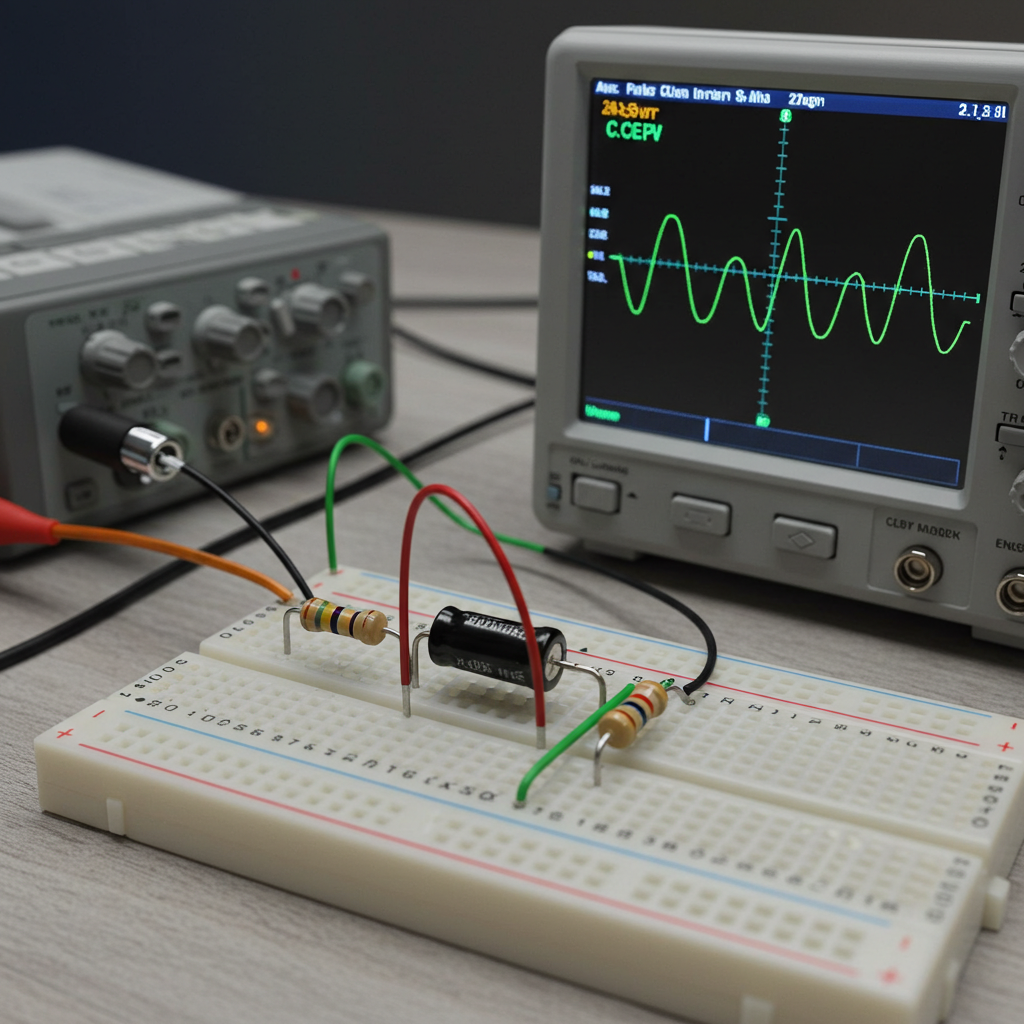
\includegraphics[width=\textwidth]{figs/ref.png}
    \label{fig:enter-label}
    \textbf{Generated by AI}
\end{figure}


% Table of Contents
\tableofcontents



% List of Figures
\listoffigures


\chapter{RC- Circuit}
\section{Set Up}
\section*{Introduction}
This document provides a step-by-step guide for setting up a simple RC circuit on a breadboard, where:
\begin{itemize}
    \item A resistor (\( R = 100\ \Omega \)) and a capacitor (\( C = 1\ \mu F \)) are connected in series.
    \item A function generator provides an AC signal across the entire circuit.
    \item An oscilloscope measures the voltage across the capacitor.
\end{itemize}

\section*{Components Required}
\begin{itemize}
    \item Breadboard
    \item Resistor: 100\( \Omega \)
    \item Capacitor: 1\( \mu F \)
    \item Function Generator
    \item Oscilloscope with probes
    \item Connecting Wires
\end{itemize}

\section*{Circuit Diagram}
\begin{figure}[H]
\centering
\begin{circuitikz}
\tikzstyle{every node}=[font=\LARGE]




% RC circuit
\draw (2.25,3.5) to[R] (4.25,3.5);
\draw (1.5,3.5) to[short] (2.25,3.5);
\draw (4.25,3.5) to[short] (5.25,3.5);
\draw (5.25,3.5) to[C] (5.25,0);
\draw (1.5,0) to[short] (5.25,0);
\draw (1.5,3.5) to[square voltage source, sources/symbol/rotate=auto] (1.5,0);

% Output terminals
\draw (5.25,3.5) to[short, -o] (7,3.5) ;
\draw (5.25,0) to[short, -o] (7,0) ;

% Labels
\node [font=\normalsize] at (3.25,2.75) {R};
\node [font=\normalsize] at (4.5,1.5) {C};
\node [font=\normalsize] at (0.5,1.75) {$V_{in}$};
\node [font=\normalsize] at (7.25,3.5) {+};
\node [font=\normalsize] at (7.25,0) {-};
\node [font=\normalsize] at (7.25,2) {$V_{out}$};

\end{circuitikz}
\end{figure}


\section*{Step-by-Step Connection Instructions}
\begin{enumerate}
    \item Place the 100\( \Omega \) resistor and the 1\( \mu F \) capacitor on the breadboard.
    \item Connect one terminal of the resistor to the positive output of the function generator.
    \item Connect the other terminal of the resistor to one terminal of the capacitor.
    \item Connect the other terminal of the capacitor to the ground of the function generator.
    \item Connect the oscilloscope probes across the capacitor:
    \begin{itemize}
        \item The positive probe to the junction between the resistor and the capacitor.
        \item The ground probe to the ground of the function generator.
    \end{itemize}
    \item Turn on the function generator and set the desired frequency and amplitude.
    \item Observe the voltage waveform across the capacitor on the oscilloscope.
\end{enumerate}

\section*{Conclusion}
This setup allows you to study the charging and discharging behavior of the capacitor in response to the applied AC signal. The oscilloscope displays the capacitor voltage, showing phase shift and amplitude variations based on the input frequency.

\section{Response to Square Wave Input}
\begin{itemize}
   \item A square wave input of frequency \( f \) and peak voltage switching between 5V and 0V is applied. The input voltage can be expressed as a piecewise function:
\begin{equation}
    V_{in}(t) = \begin{cases} 
        5V, & 0 \leq t < T/2 \\
        0V, & T/2 \leq t < T
    \end{cases}
\end{equation}
where \( T = \frac{1}{f} \) is the period of the square wave.
\item The voltage across the capacitor follows the charging and discharging equations:
\begin{equation}
    V_C(t) = \begin{cases} 
        5(1 - e^{-t/\tau}), & 0 \leq t < T/2 \\
        V_C(T/2) e^{-(t-T/2)/\tau}, & T/2 \leq t < T
    \end{cases}
\end{equation}
where \( \tau = RC \) is the time constant of the circuit.

   \item  At the end of each half-cycle, the capacitor voltage reaches:
\begin{equation}
    V_C(T/2) = 5(1 - e^{-T/2\tau})
\end{equation}
for the charging phase and
\begin{equation}
    V_C(T) = V_C(T/2) e^{-T/2\tau}
\end{equation}
for the discharging phase.

   \item This theoretical derivation shows the capacitor voltage exhibits an exponential rise and fall pattern, rather than an abrupt transition.

\end{itemize}
\section*{Transient and Steady-State Response}
The response of an RC circuit can be divided into two phases:
\begin{itemize}
    \item \textbf{Transient Response:} This occurs immediately after a change in input voltage. It represents the period where the capacitor voltage is adjusting and follows an exponential rise or decay.
    \begin{equation}
        V_C(t) = V_f + (V_i - V_f) e^{-t/\tau}
    \end{equation}
     where \( V_i \) is the initial voltage, \( V_f \) is the final voltage the capacitor attempts to reach, and \( \tau = RC \) is the time constant.
   
    
    \item \textbf{Steady-State Response:} This occurs when sufficient time has passed, and the capacitor voltage no longer changes significantly with time. For a periodic input like a square wave, the capacitor voltage oscillates between fixed values without further long-term variation.
\end{itemize}

The transition from transient to steady-state depends on the time constant \( \tau \), with a common rule of thumb being that the transient phase lasts about \( 5\tau \), after which the circuit is considered to have reached steady state.

\section{Results}
\subsection{$RC = T$}
\begin{itemize}
    \item Transient response:
    \begin{figure}[H] % H forces the figure to be placed exactly here
    \centering
    % Replace "1.jpg" with your actual image filename
    \begin{minipage}[c]{0.48\textwidth}
        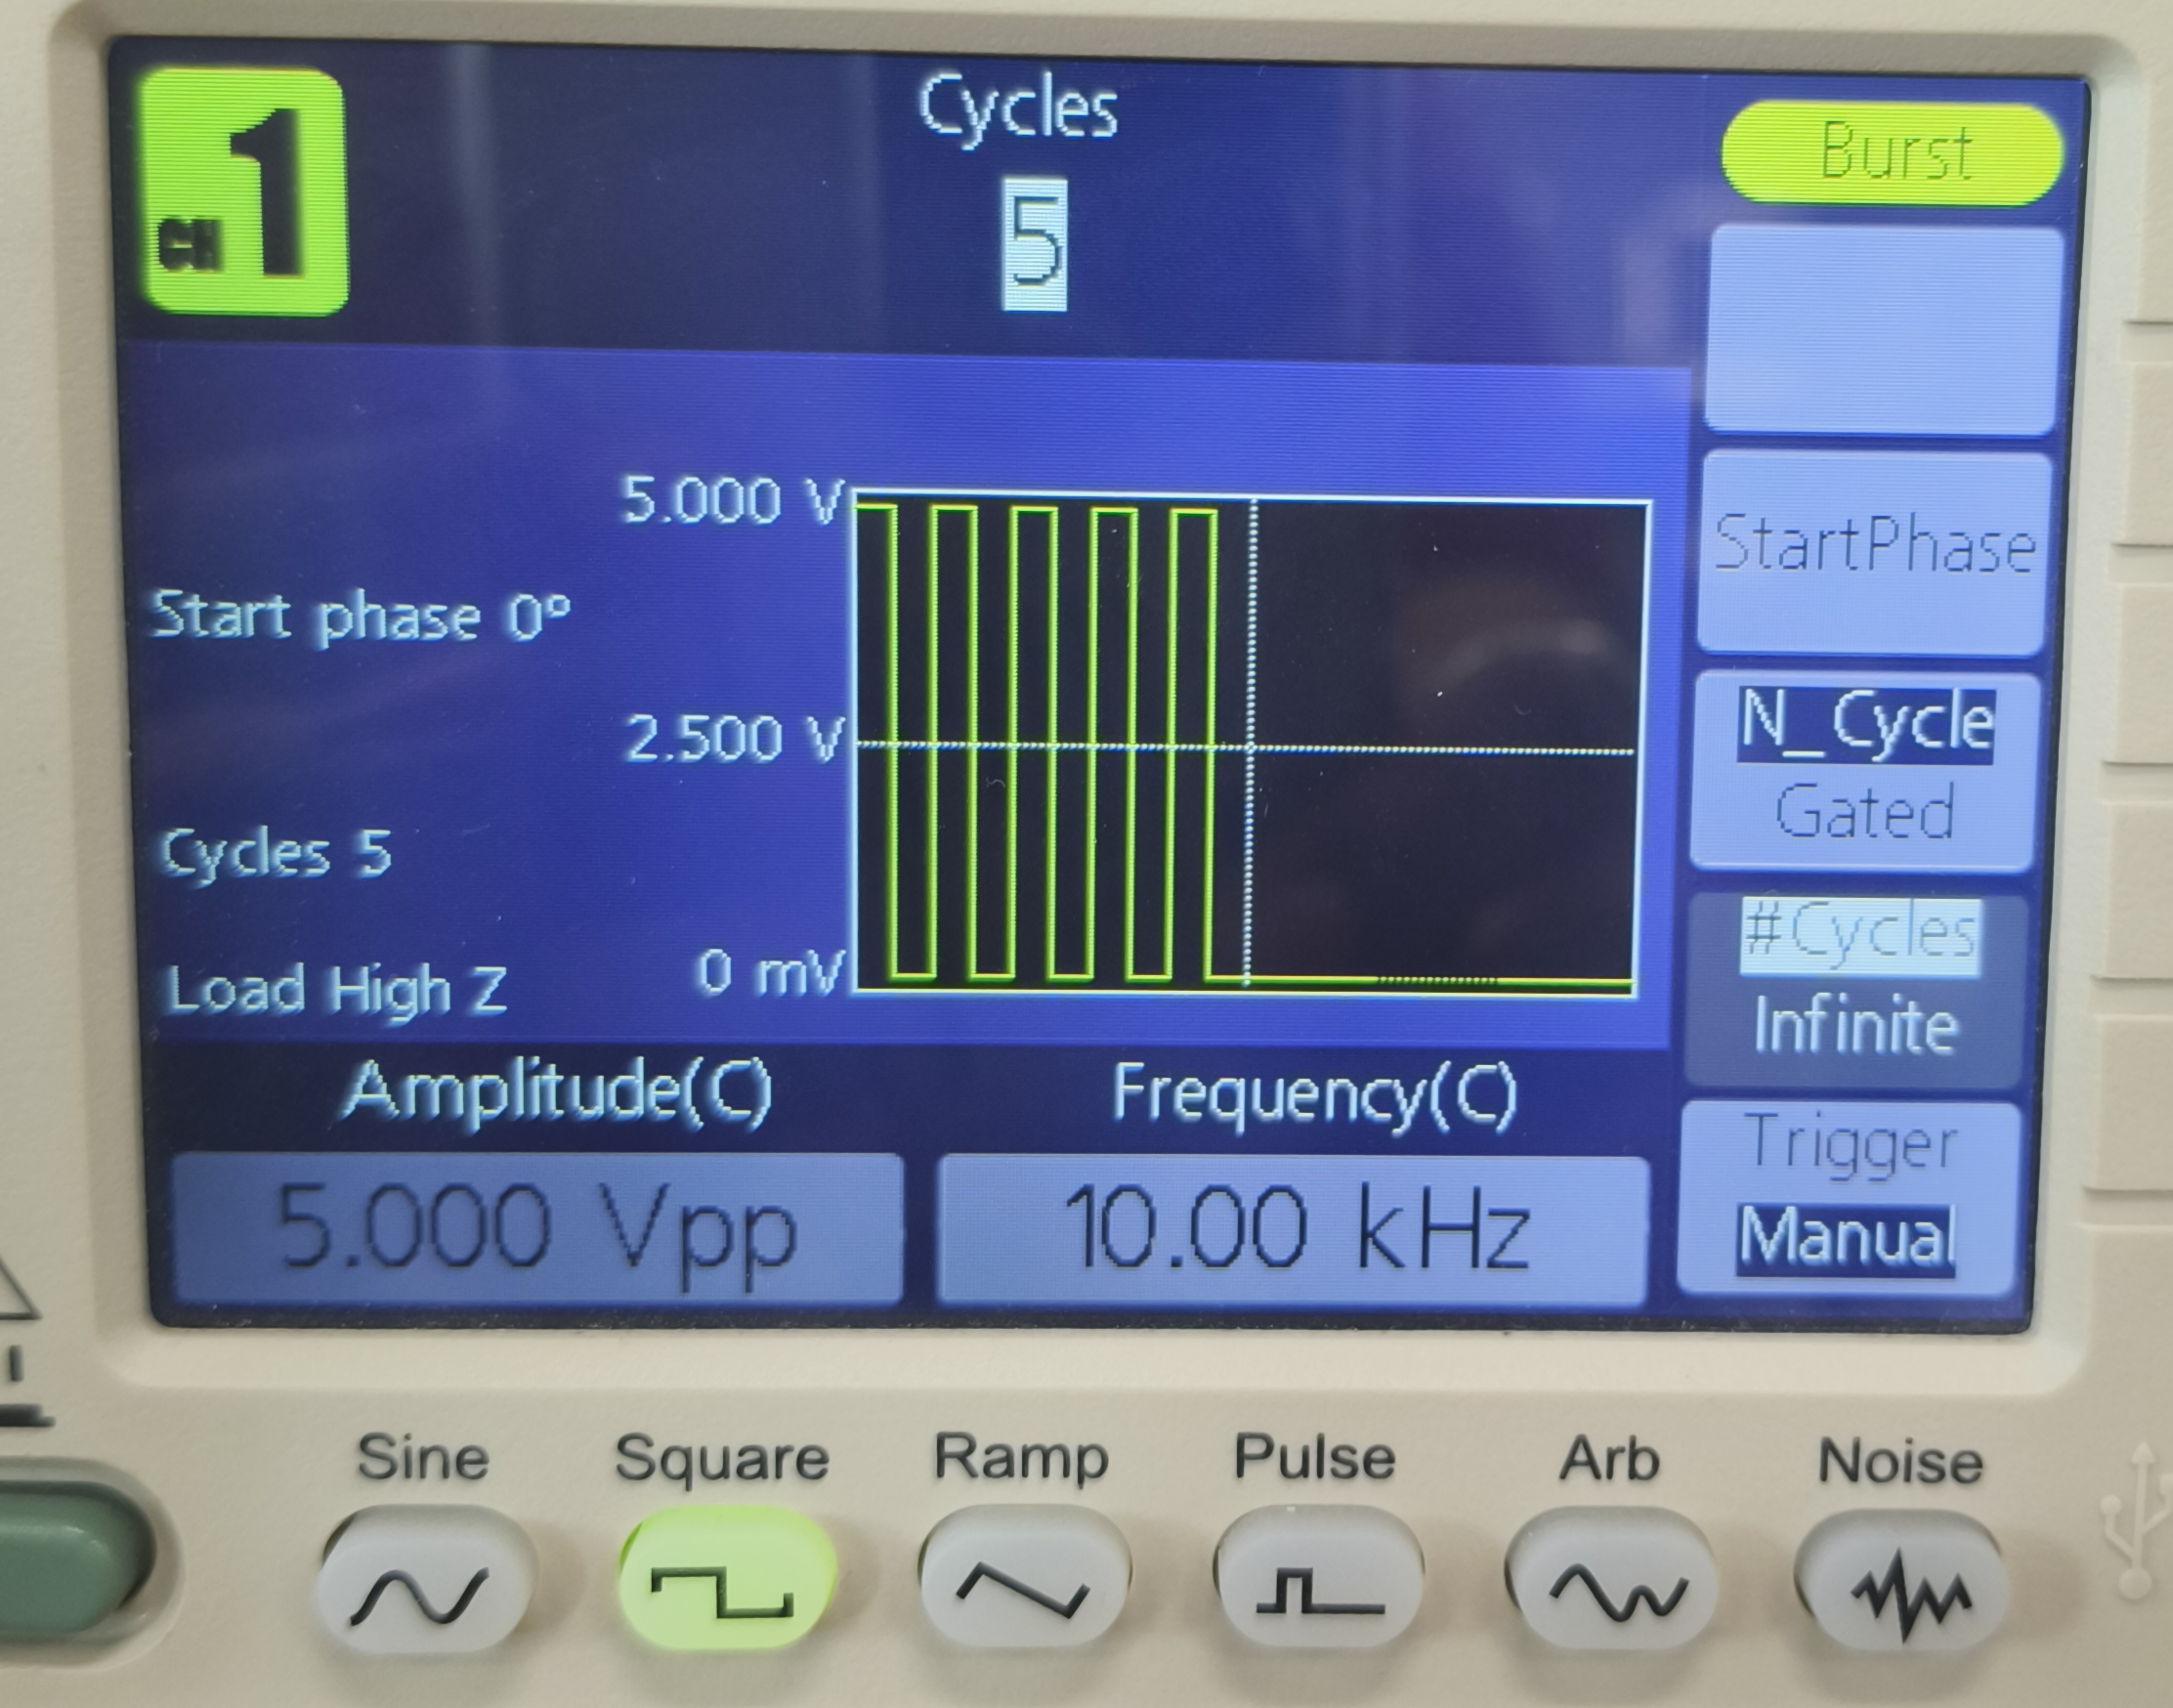
\includegraphics[width=\textwidth]{figs/t1.jpg} % Replace with the actual file name
        
    \end{minipage}
    \hfill
    \begin{minipage}[c]{0.48\textwidth}
        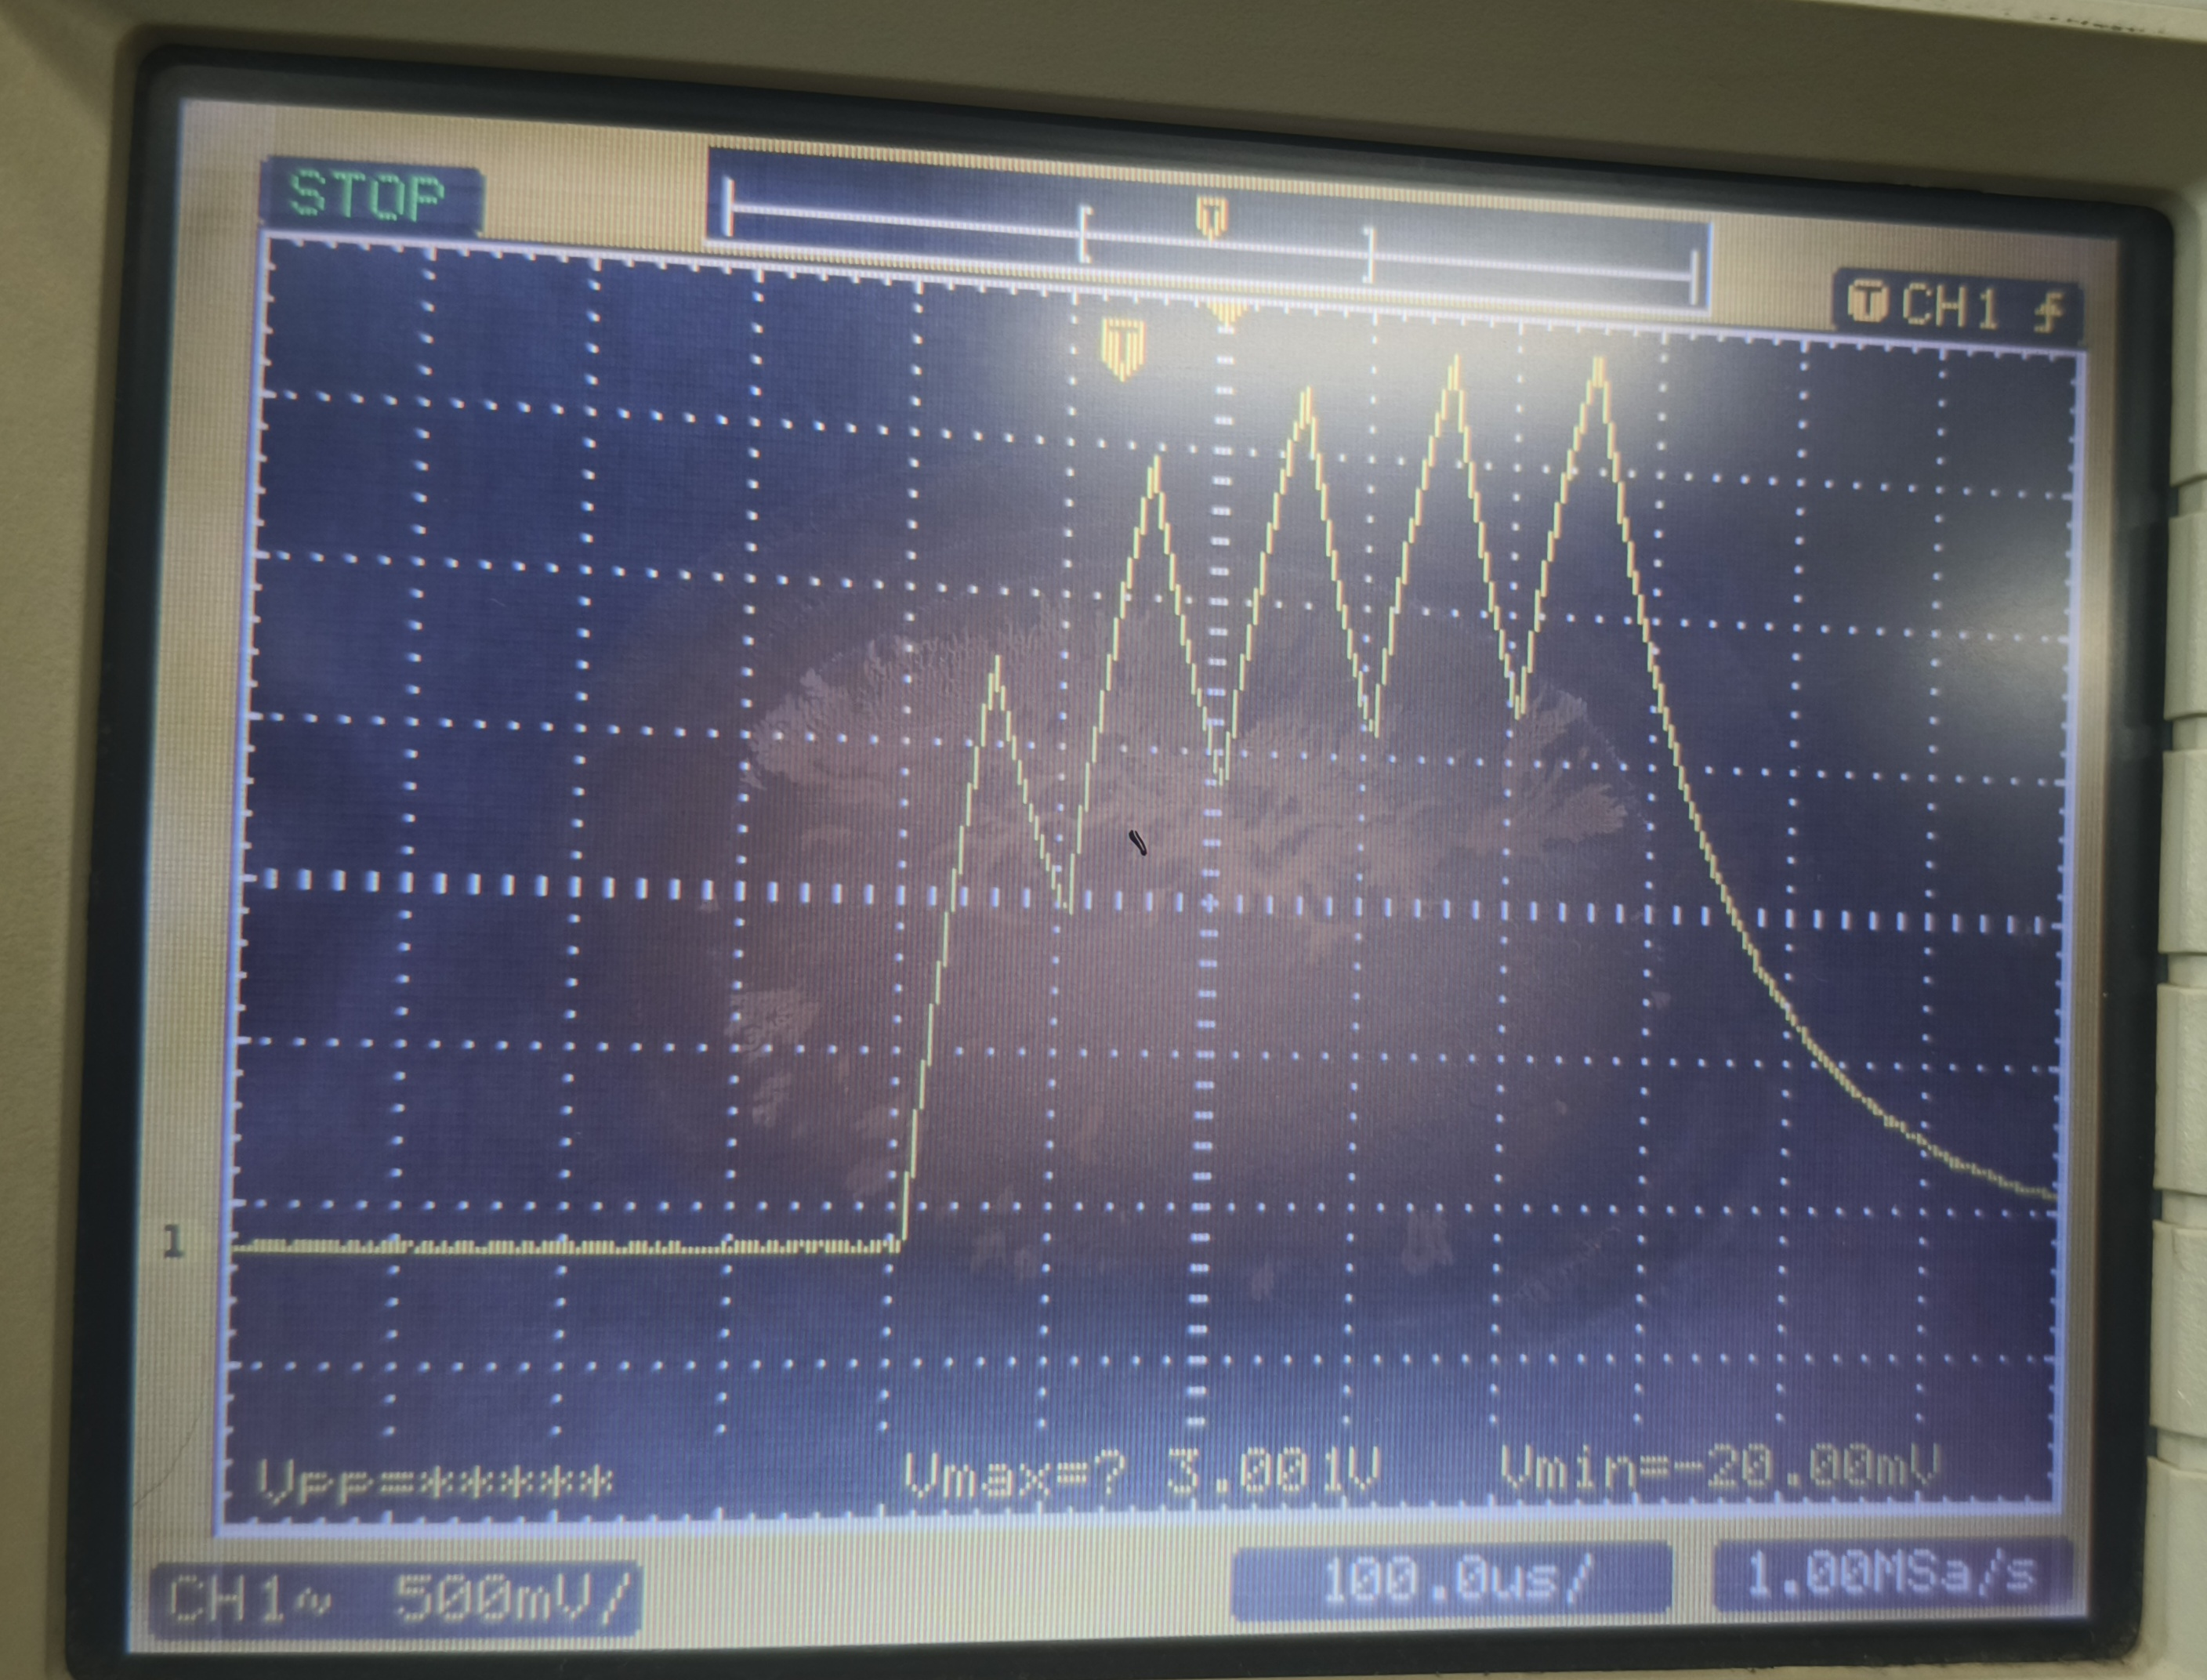
\includegraphics[width=\textwidth]{figs/tr1.jpg} % Replace with the actual file name
        
    \end{minipage}
    \caption{Transient RC=T}
    \label{fig:CRO-patterns}
\end{figure}
\begin{figure}
    \centering
    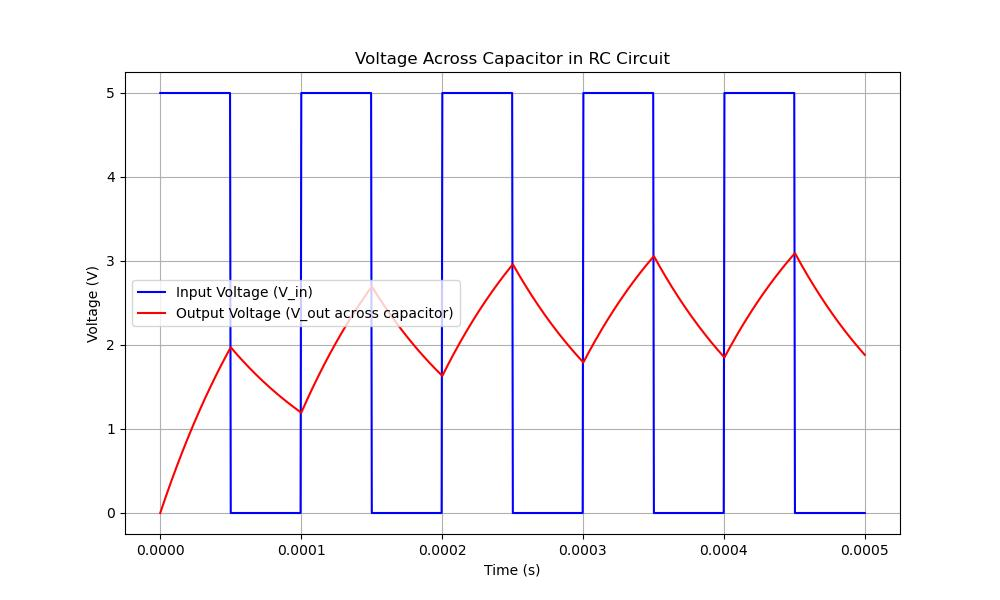
\includegraphics[width=\textwidth]{figs/1.jpg}
    \caption{Python RC = T}
    \label{fig:enter-label}
\end{figure}
    \item Steady-state response:
    \begin{figure}[H] % H forces the figure to be placed exactly here
    \centering
    % Replace "1.jpg" with your actual image filename
    \begin{minipage}[c]{0.48\textwidth}
        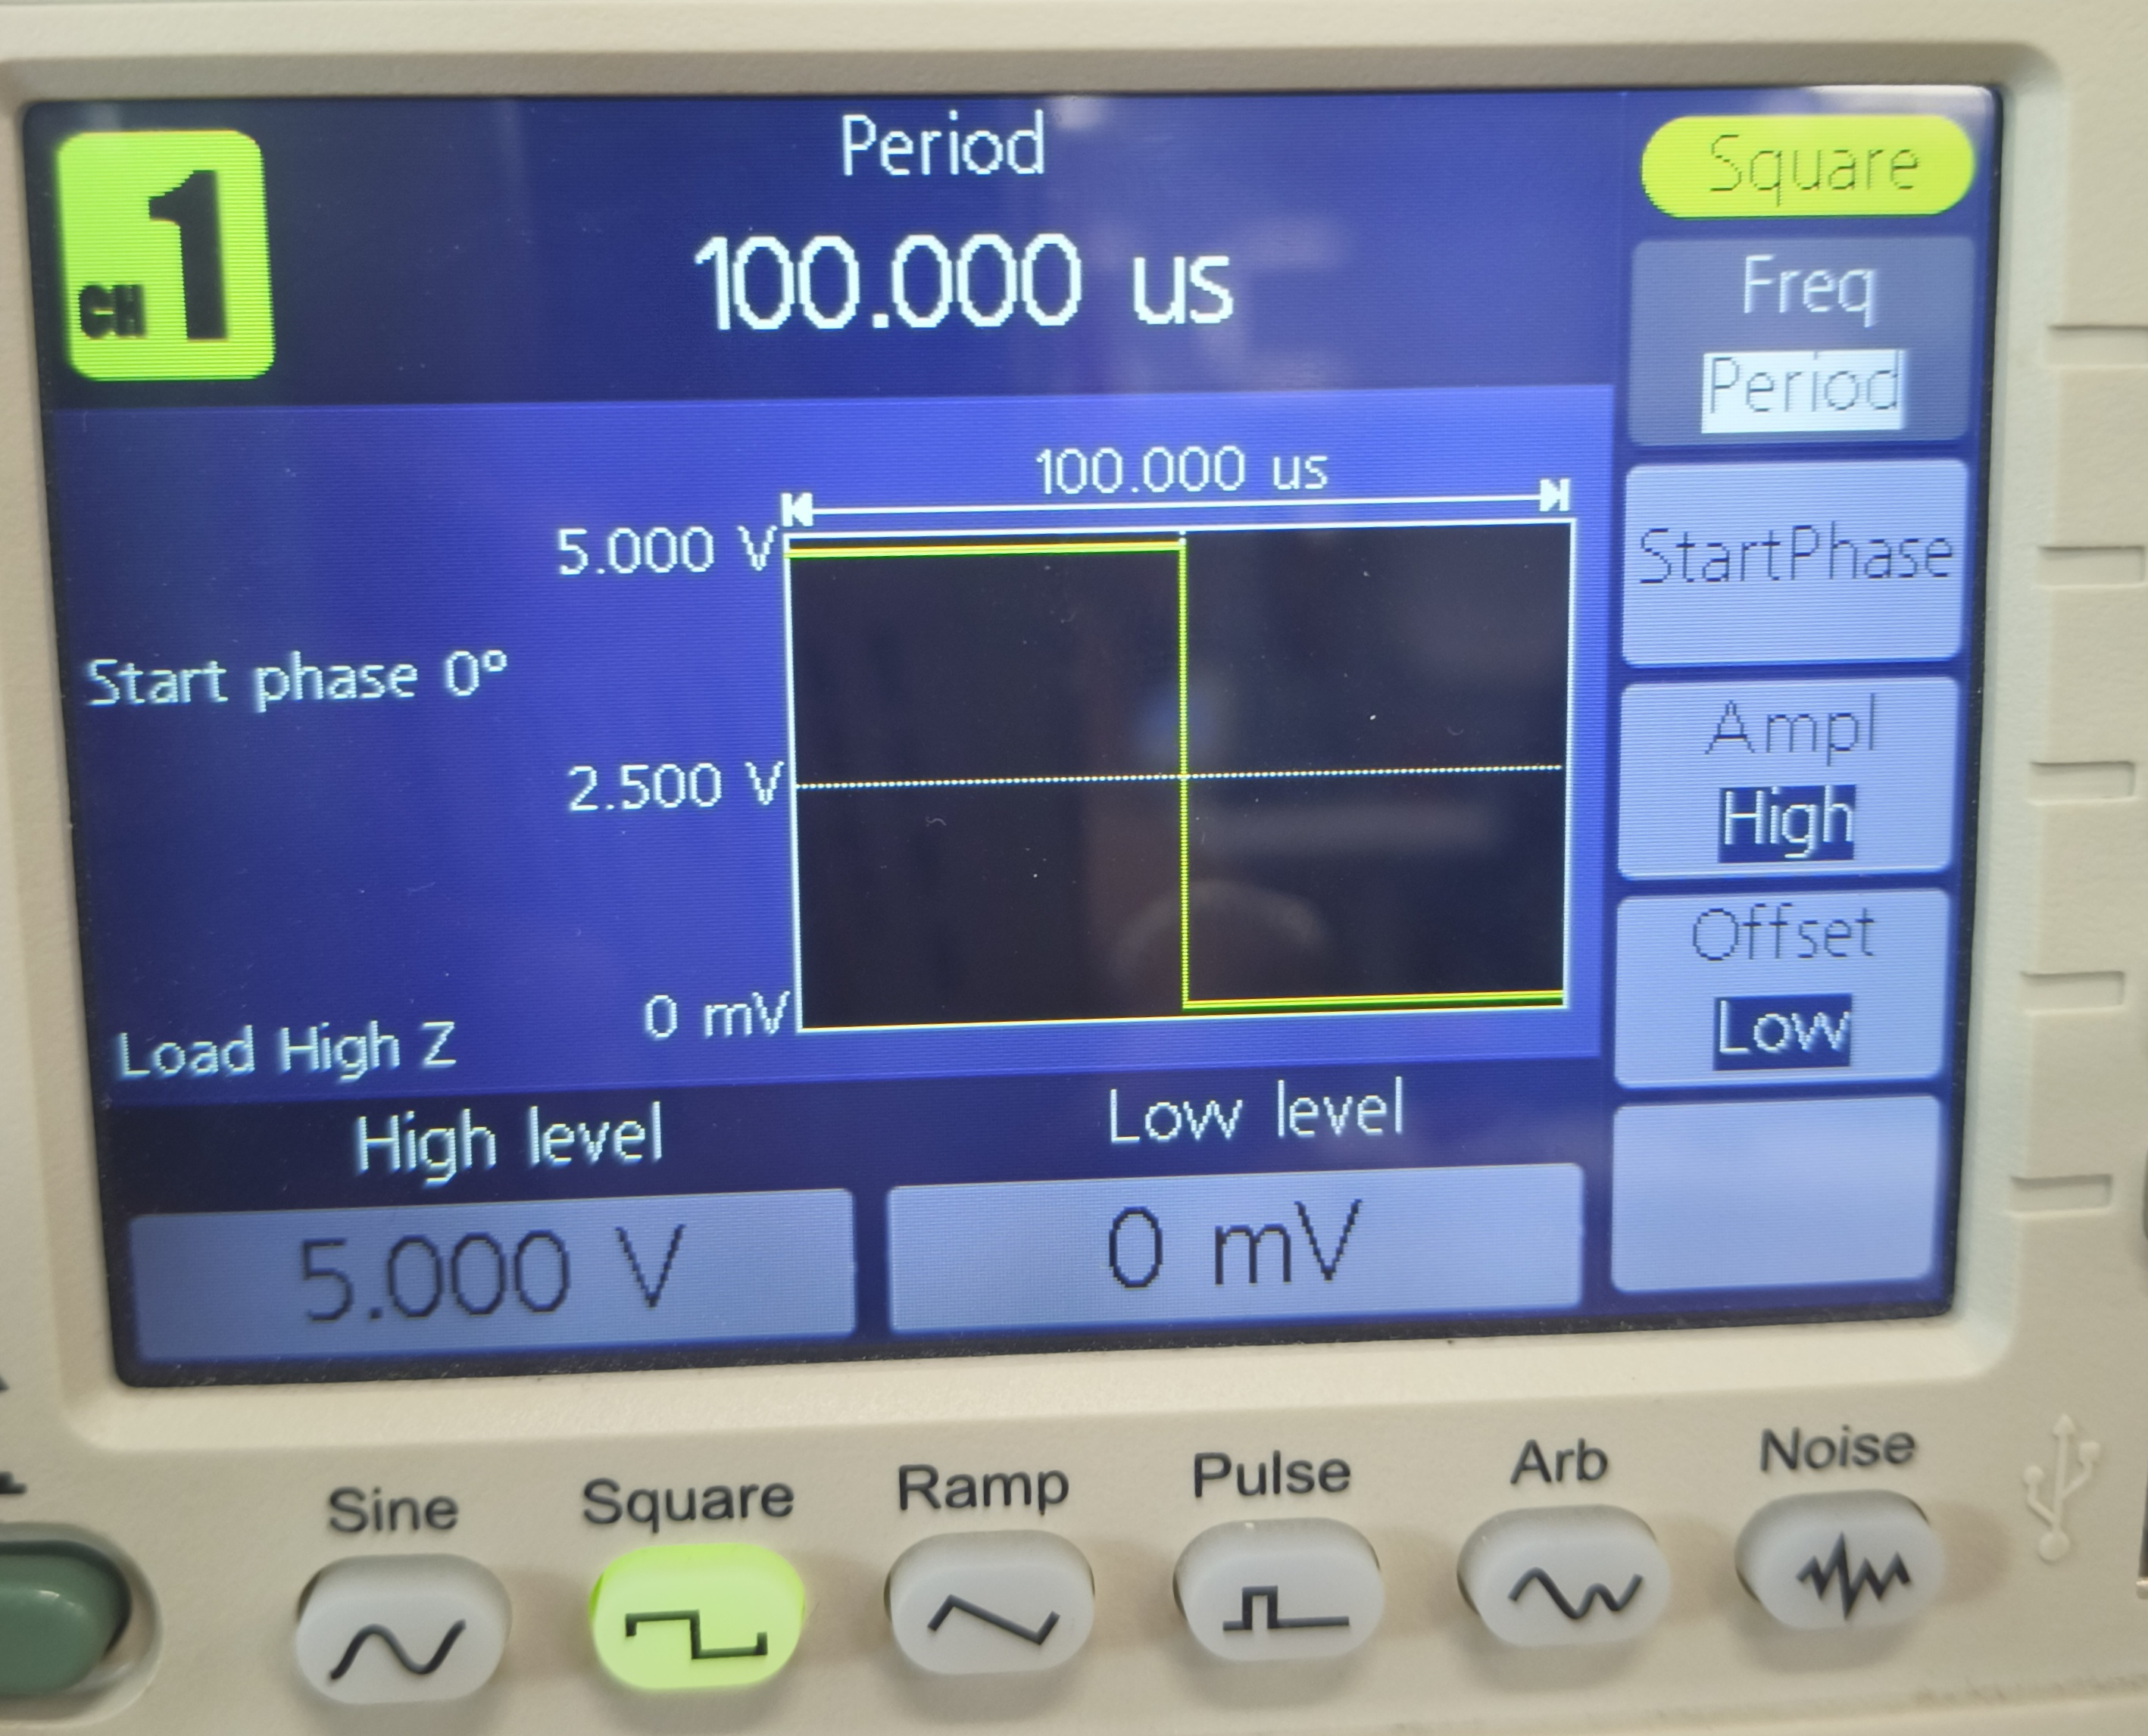
\includegraphics[width=\textwidth]{figs/s1.jpg} % Replace with the actual file name
        
    \end{minipage}
    \hfill
    \begin{minipage}[c]{0.48\textwidth}
        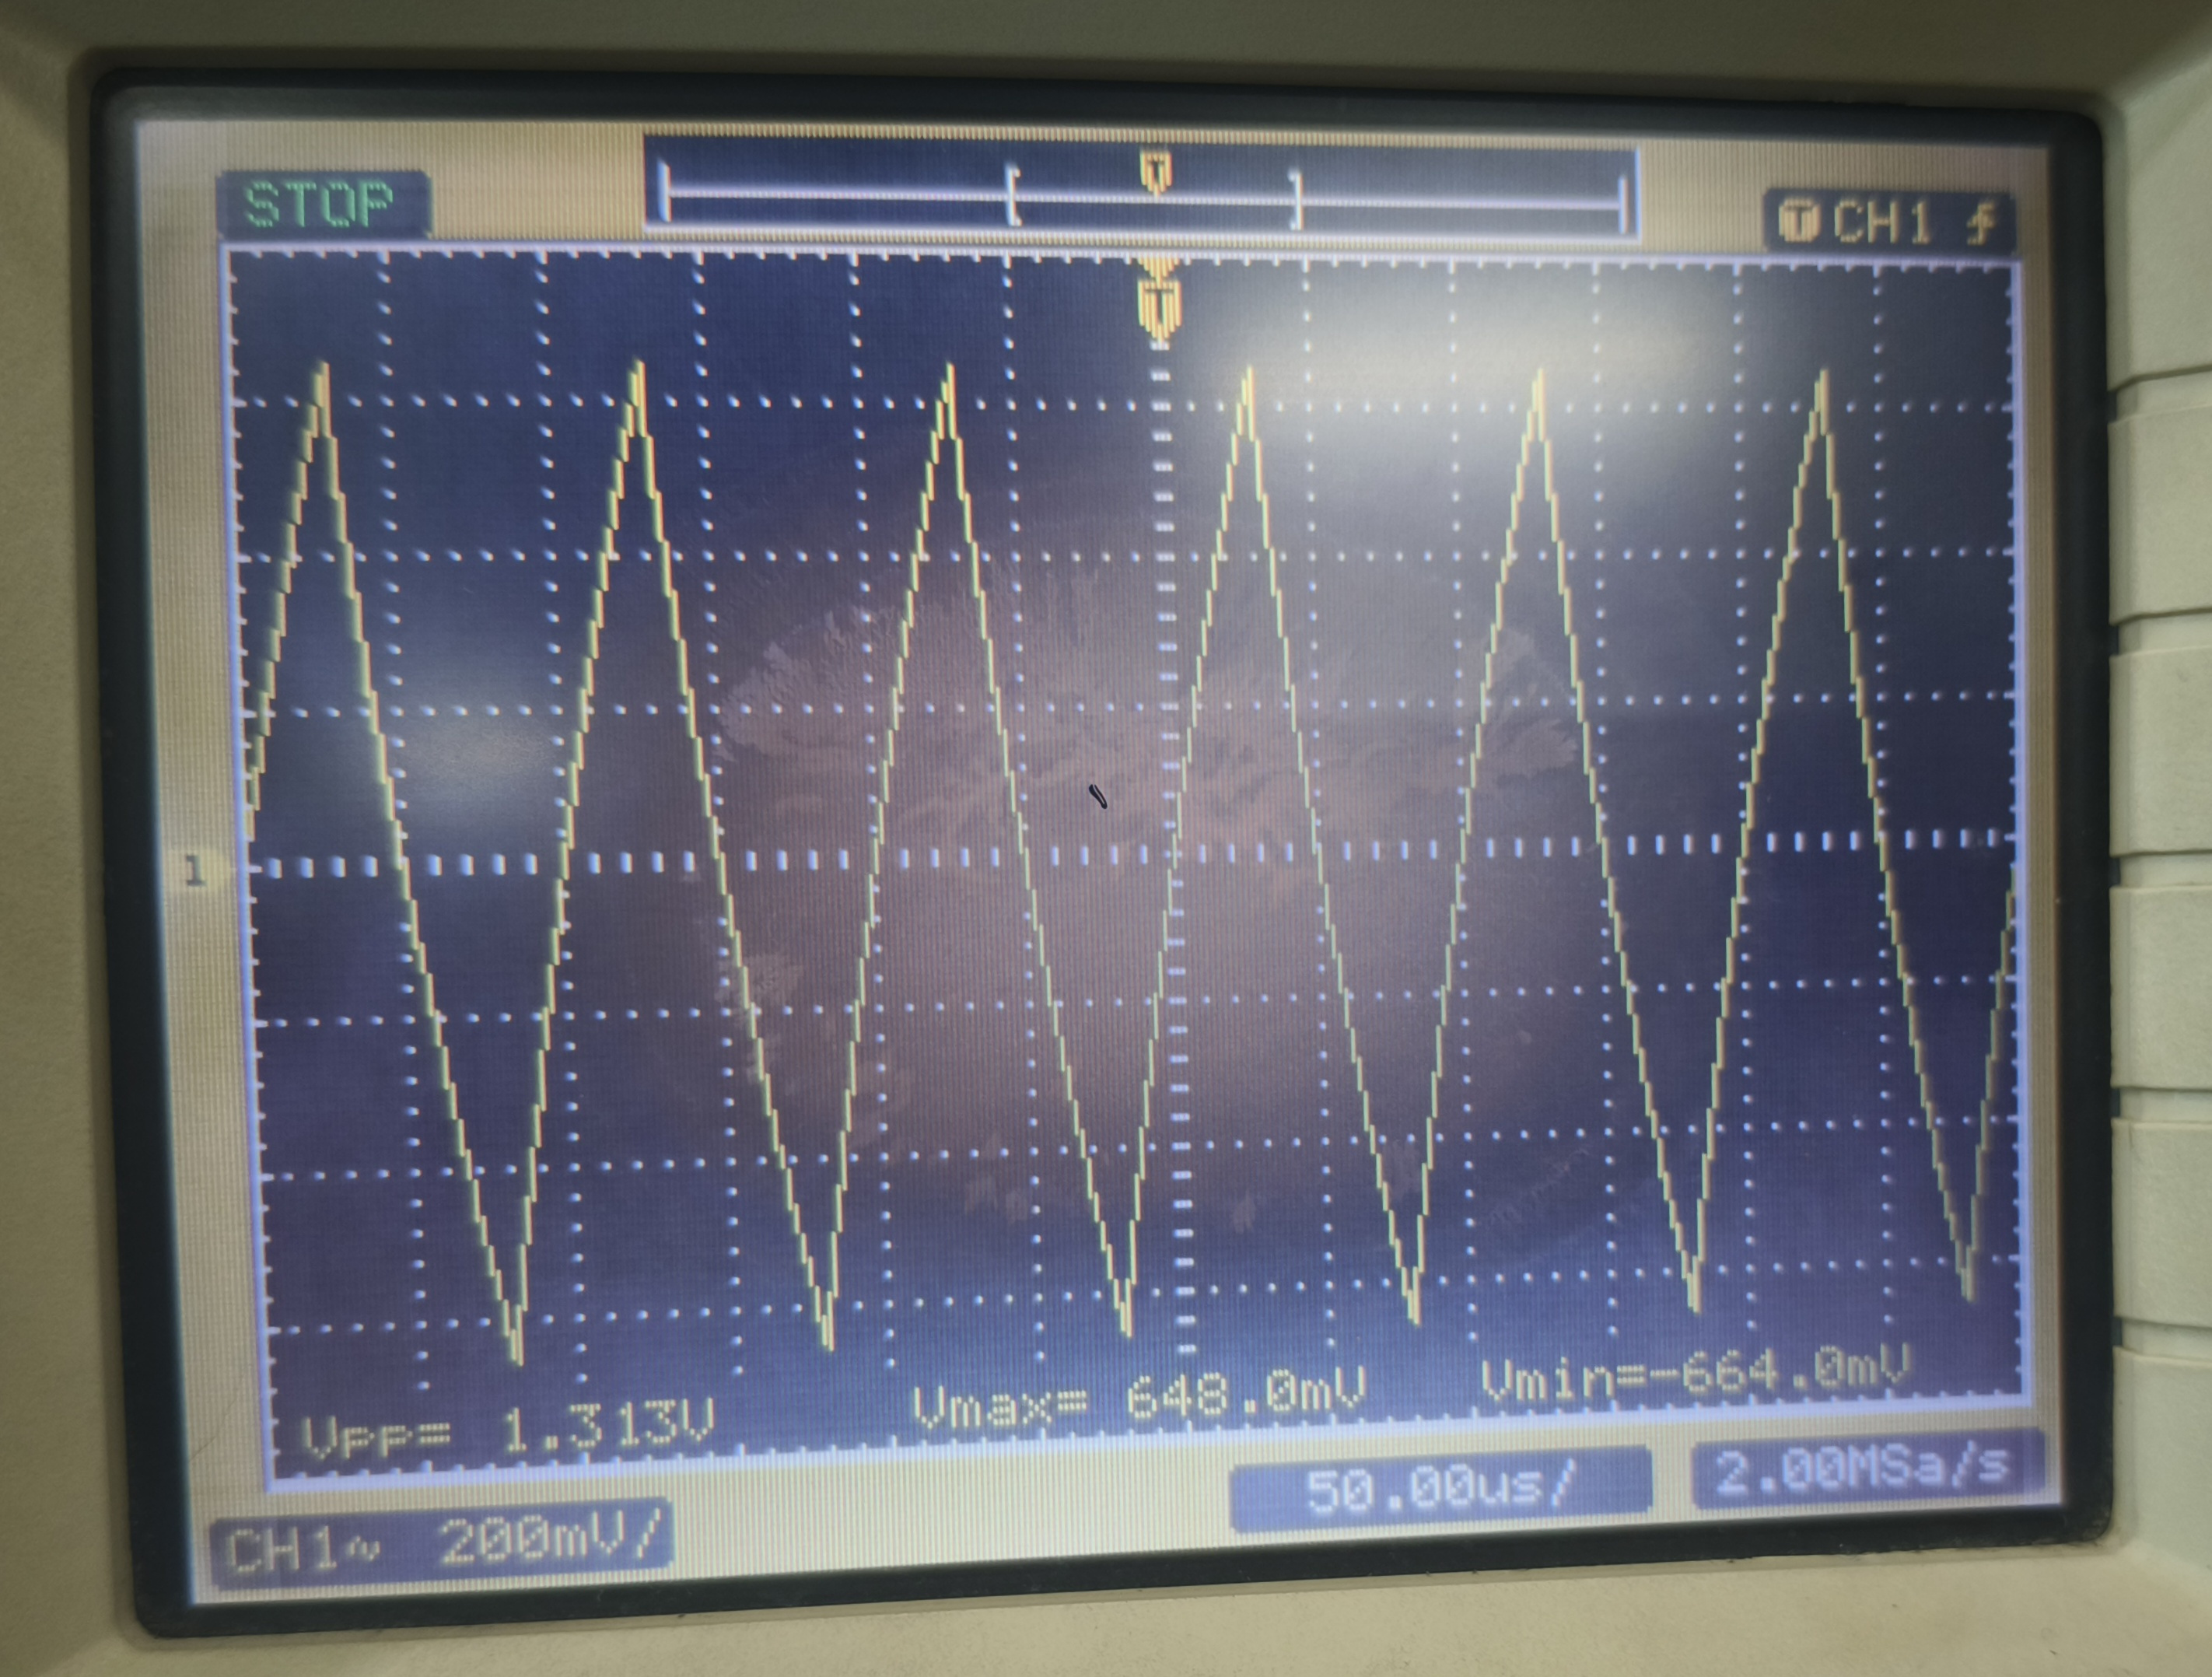
\includegraphics[width=\textwidth]{figs/sr1.jpg} % Replace with the actual file name
        
    \end{minipage}
    \caption{Steady State RC=T}
    \label{fig:CRO-patterns}
\end{figure}
\end{itemize}

\subsection{$RC \ll T$}
\begin{itemize}
    \item Transient response:
    \begin{figure}[H] % H forces the figure to be placed exactly here
    \centering
    % Replace "1.jpg" with your actual image filename
    \begin{minipage}[c]{0.48\textwidth}
        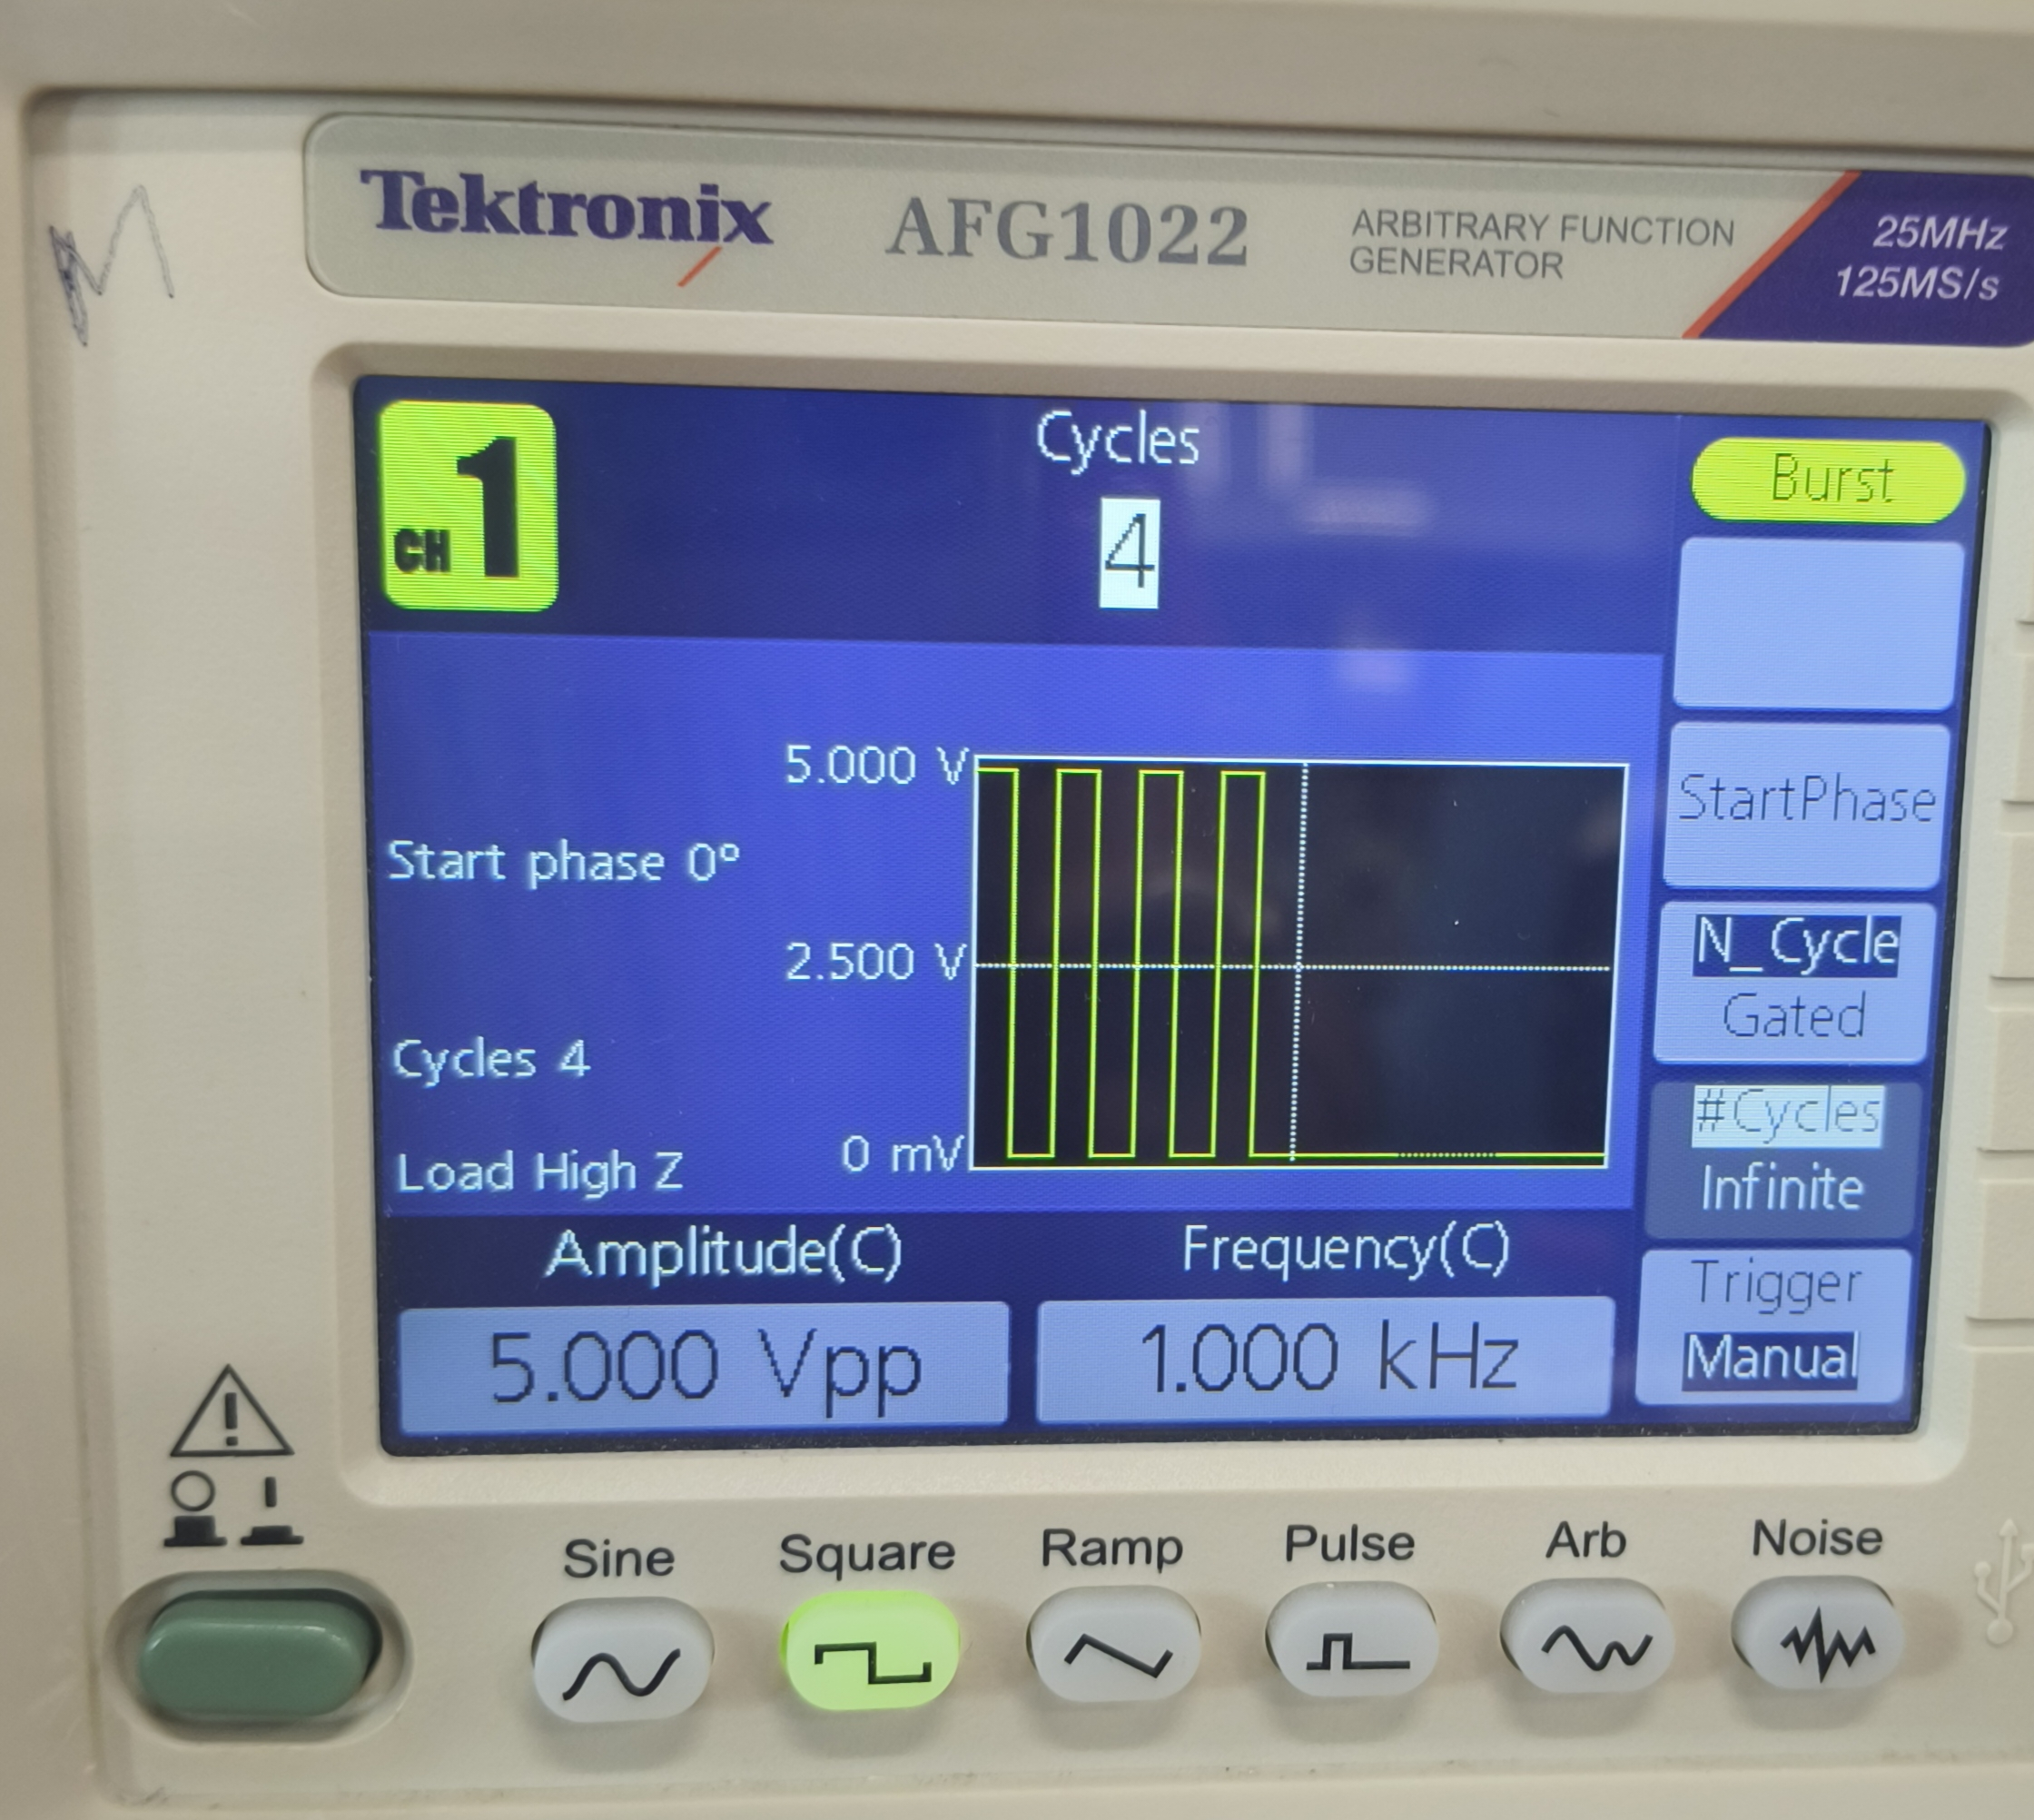
\includegraphics[width=\textwidth]{figs/t2.jpg} % Replace with the actual file name
        
    \end{minipage}
    \hfill
    \begin{minipage}[c]{0.48\textwidth}
        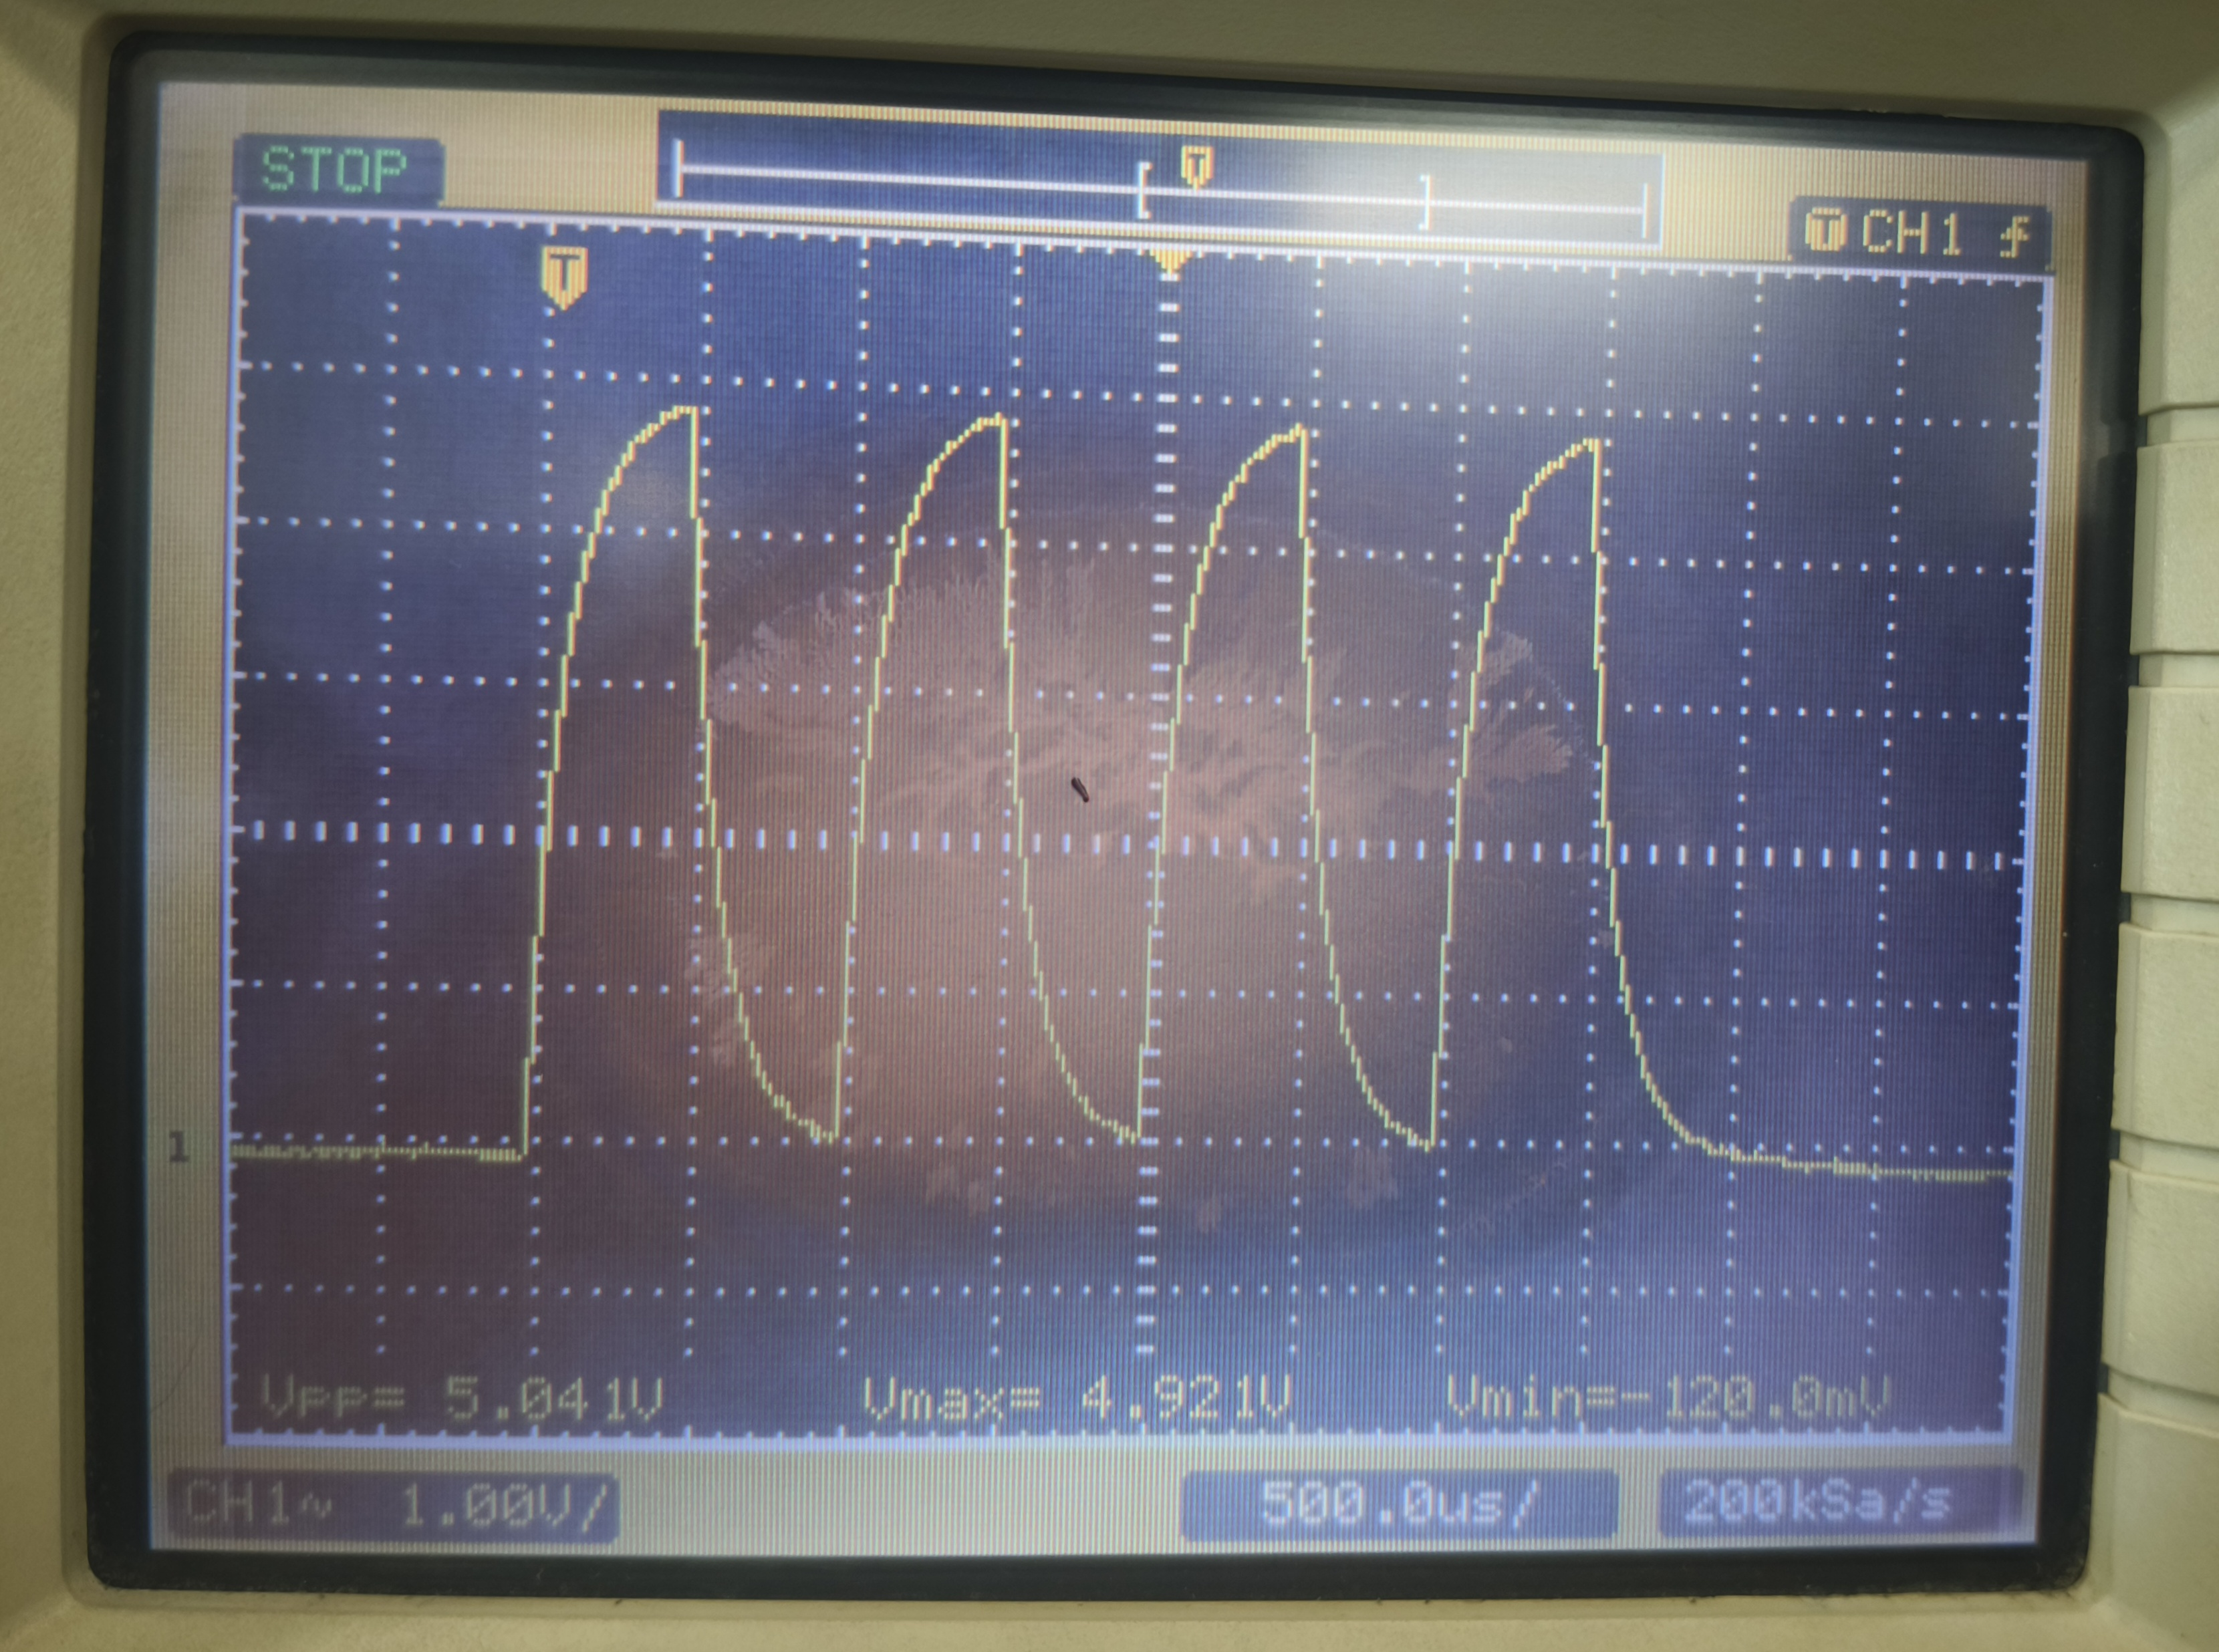
\includegraphics[width=\textwidth]{figs/tr2.jpg} % Replace with the actual file name
        
    \end{minipage}
    \caption{Transient $RC \ll T$}
    \label{fig:CRO-patterns}
\end{figure}
\begin{figure}
    \centering
    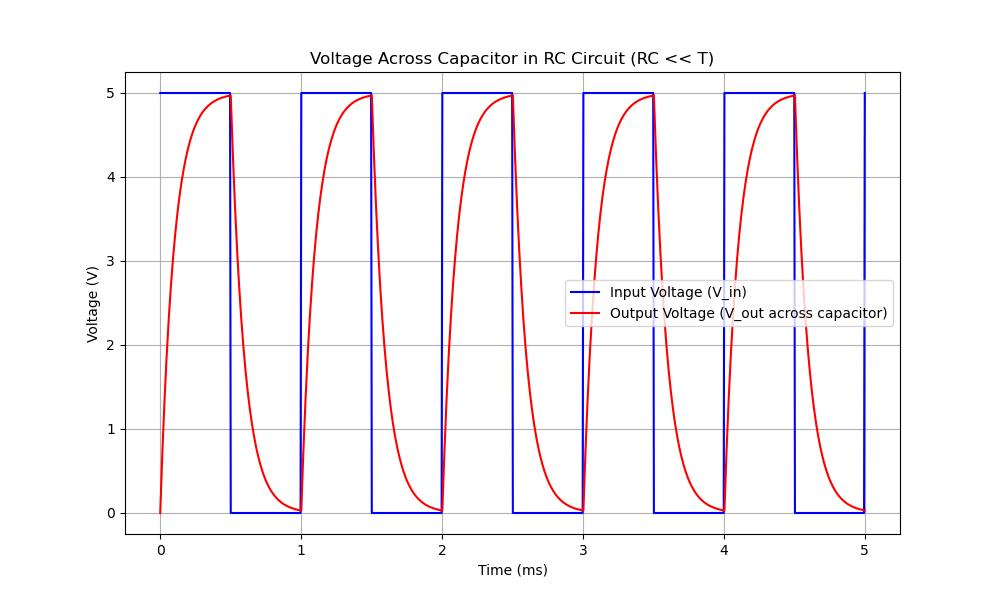
\includegraphics[width=\textwidth]{figs/2.jpg}
    \caption{Python $RC \ll T$}
    \label{fig:enter-label}
\end{figure}
    \item Steady-state response:
    \begin{figure}[H] % H forces the figure to be placed exactly here
    \centering
    % Replace "1.jpg" with your actual image filename
    \begin{minipage}[c]{0.48\textwidth}
        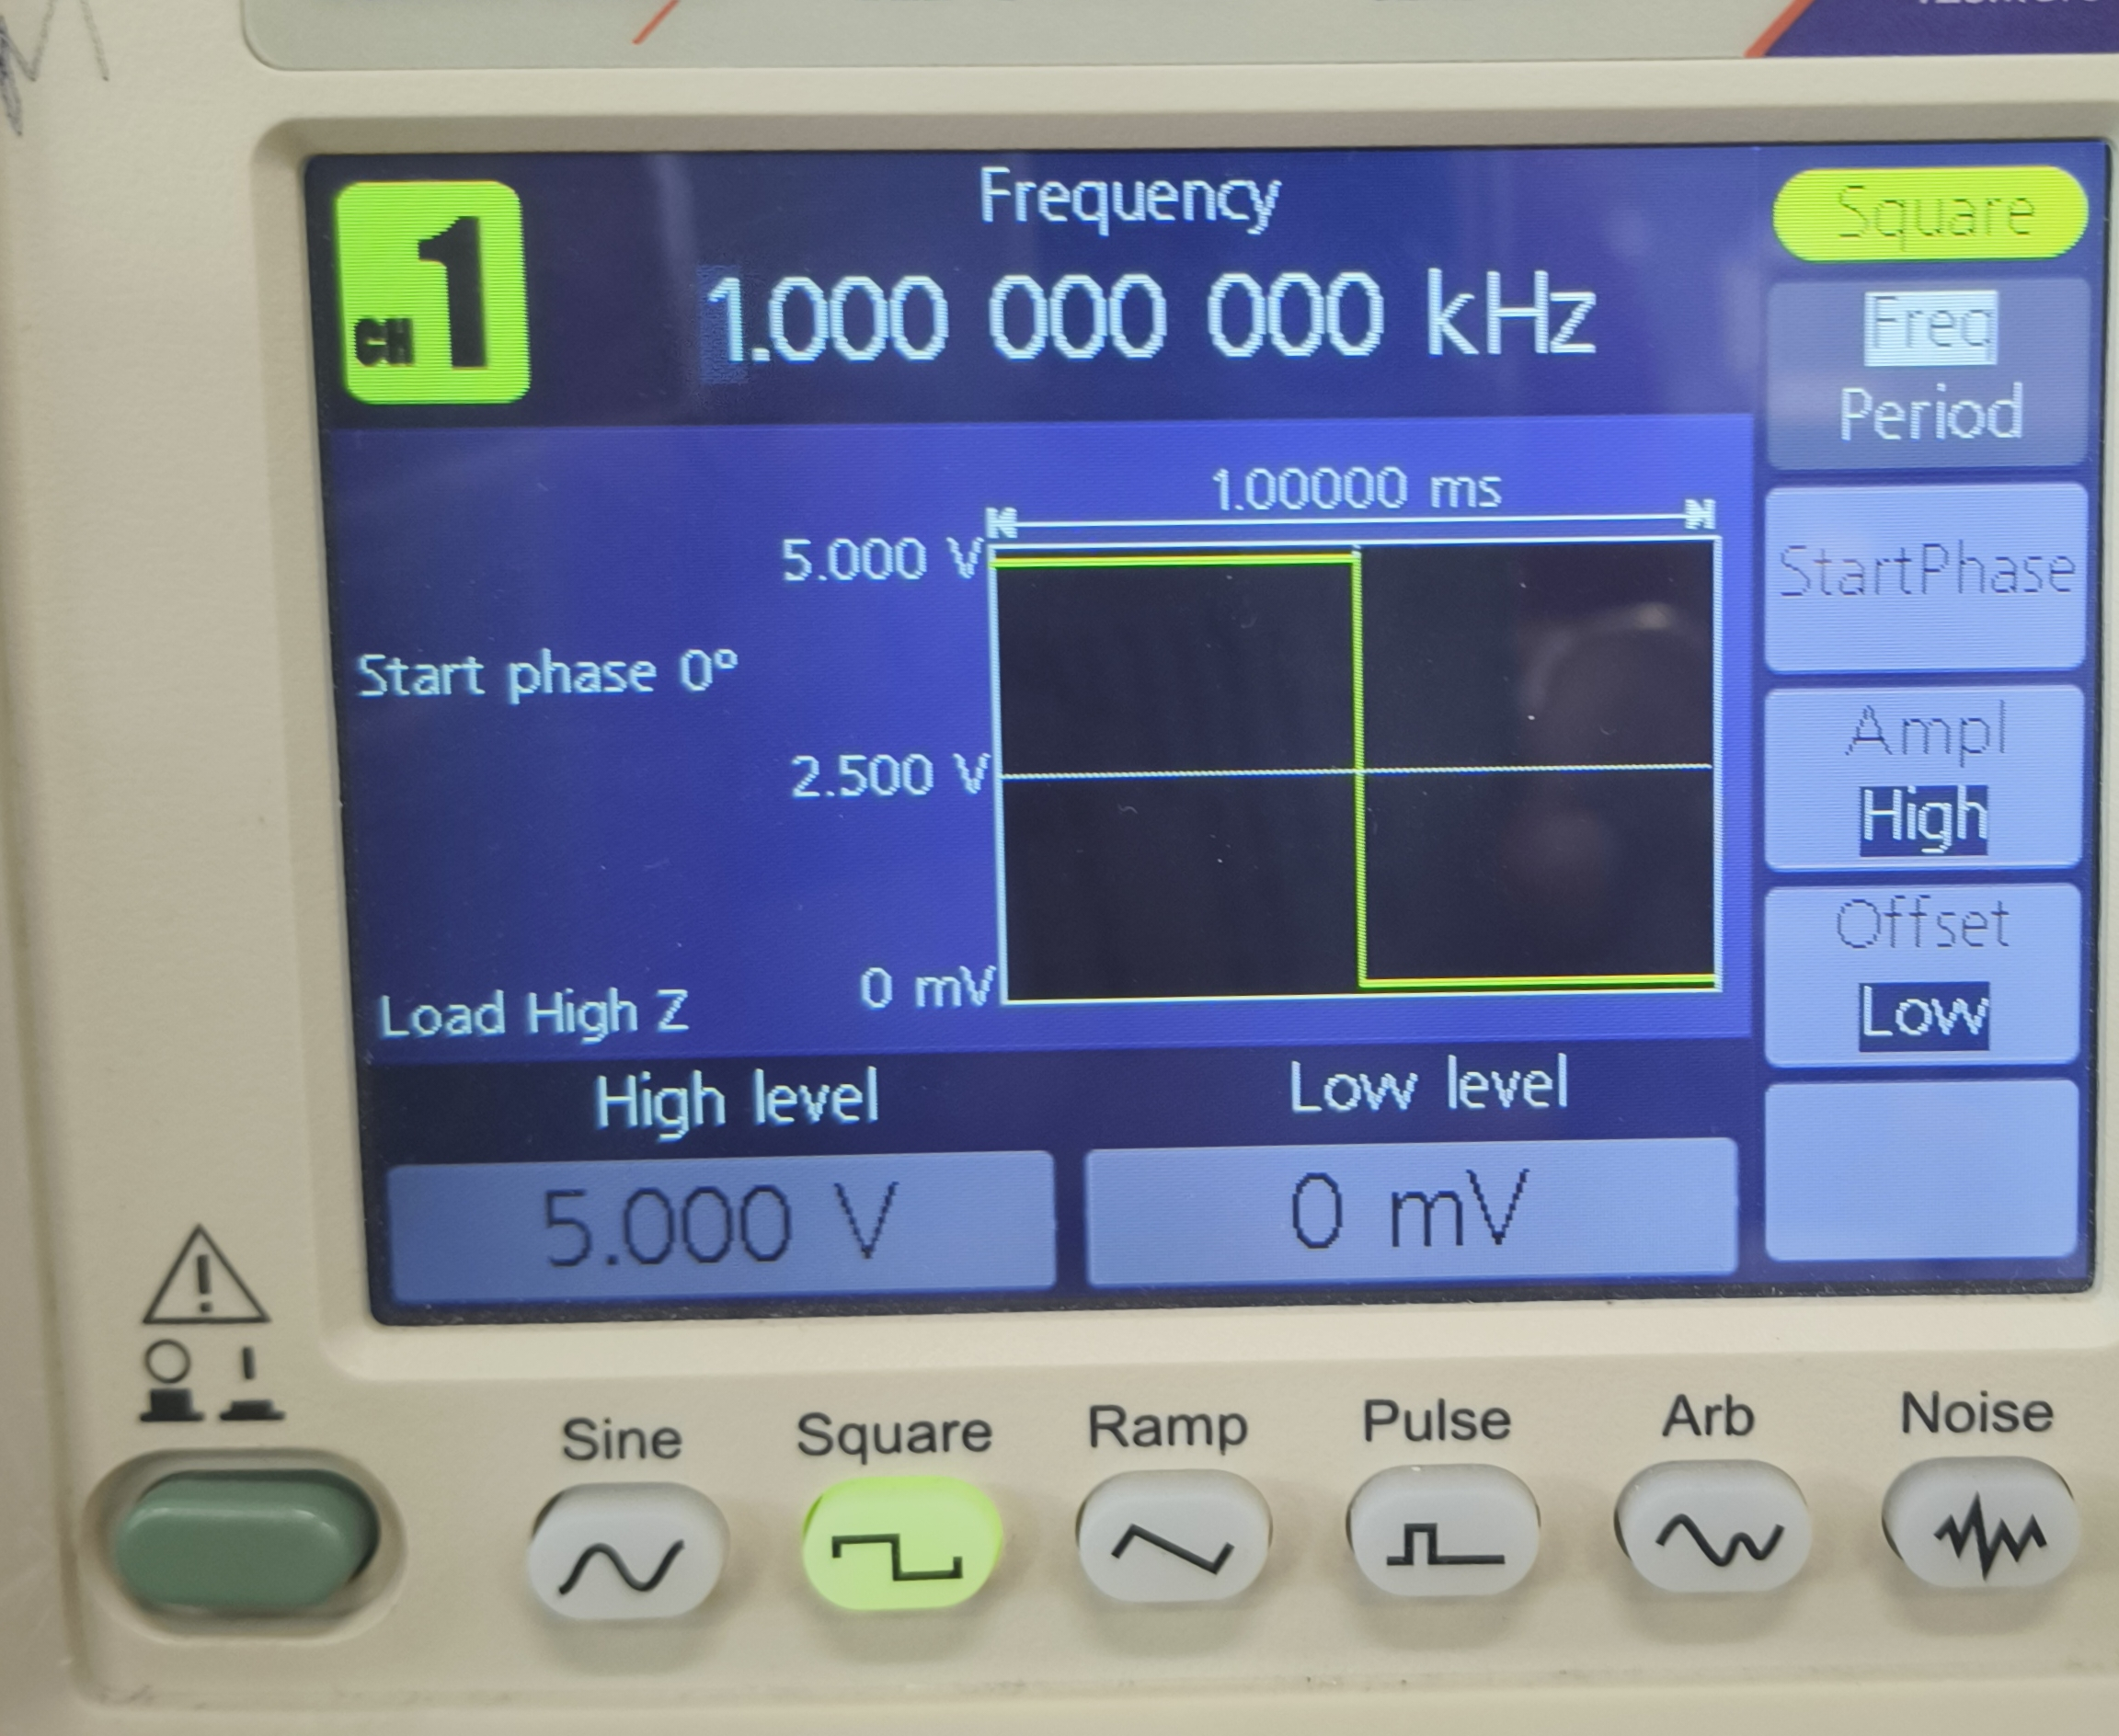
\includegraphics[width=\textwidth]{figs/s2.jpg} % Replace with the actual file name
        
    \end{minipage}
    \hfill
    \begin{minipage}[c]{0.48\textwidth}
        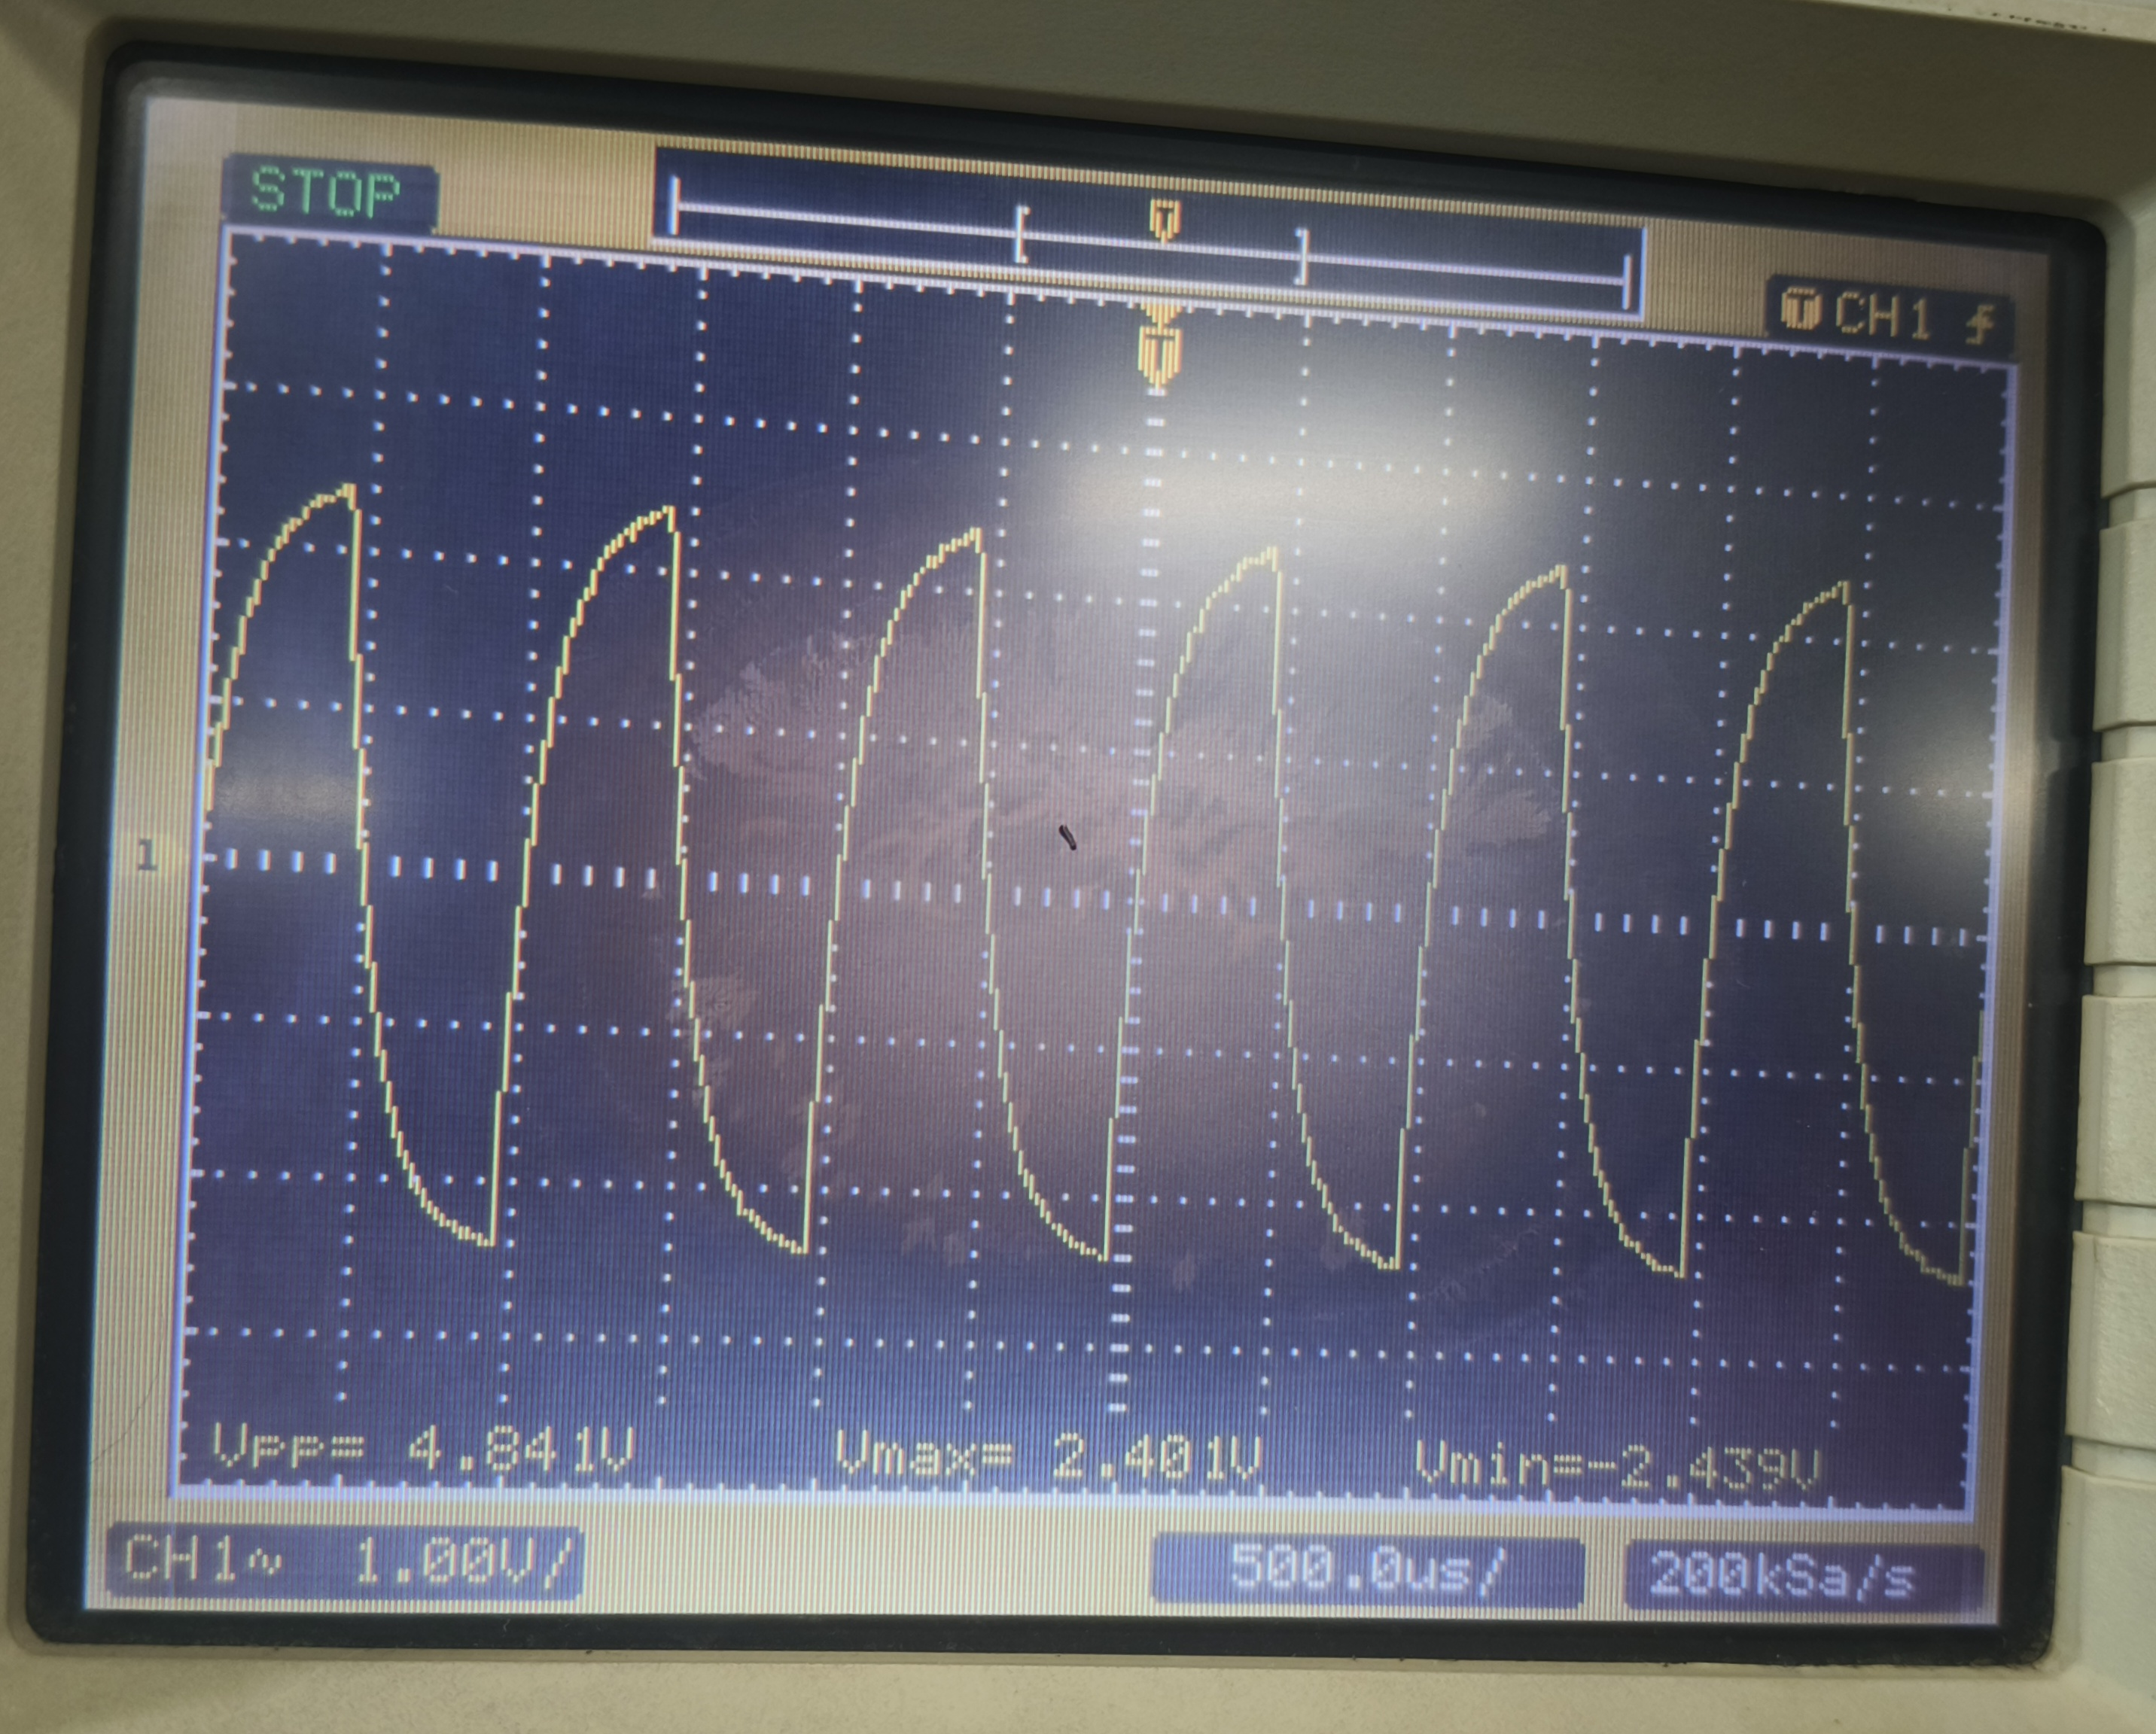
\includegraphics[width=\textwidth]{figs/sr2.jpg} % Replace with the actual file name
        
    \end{minipage}
    \caption{Steady State $RC \ll T$}
    \label{fig:CRO-patterns}
\end{figure}
\end{itemize}

\subsection{$RC \gg T$}
\begin{itemize}
    \item Transient response: For Finite Cycles
    \begin{figure}[H] % H forces the figure to be placed exactly here
    \centering
    % Replace "1.jpg" with your actual image filename
    \begin{minipage}[c]{0.48\textwidth}
        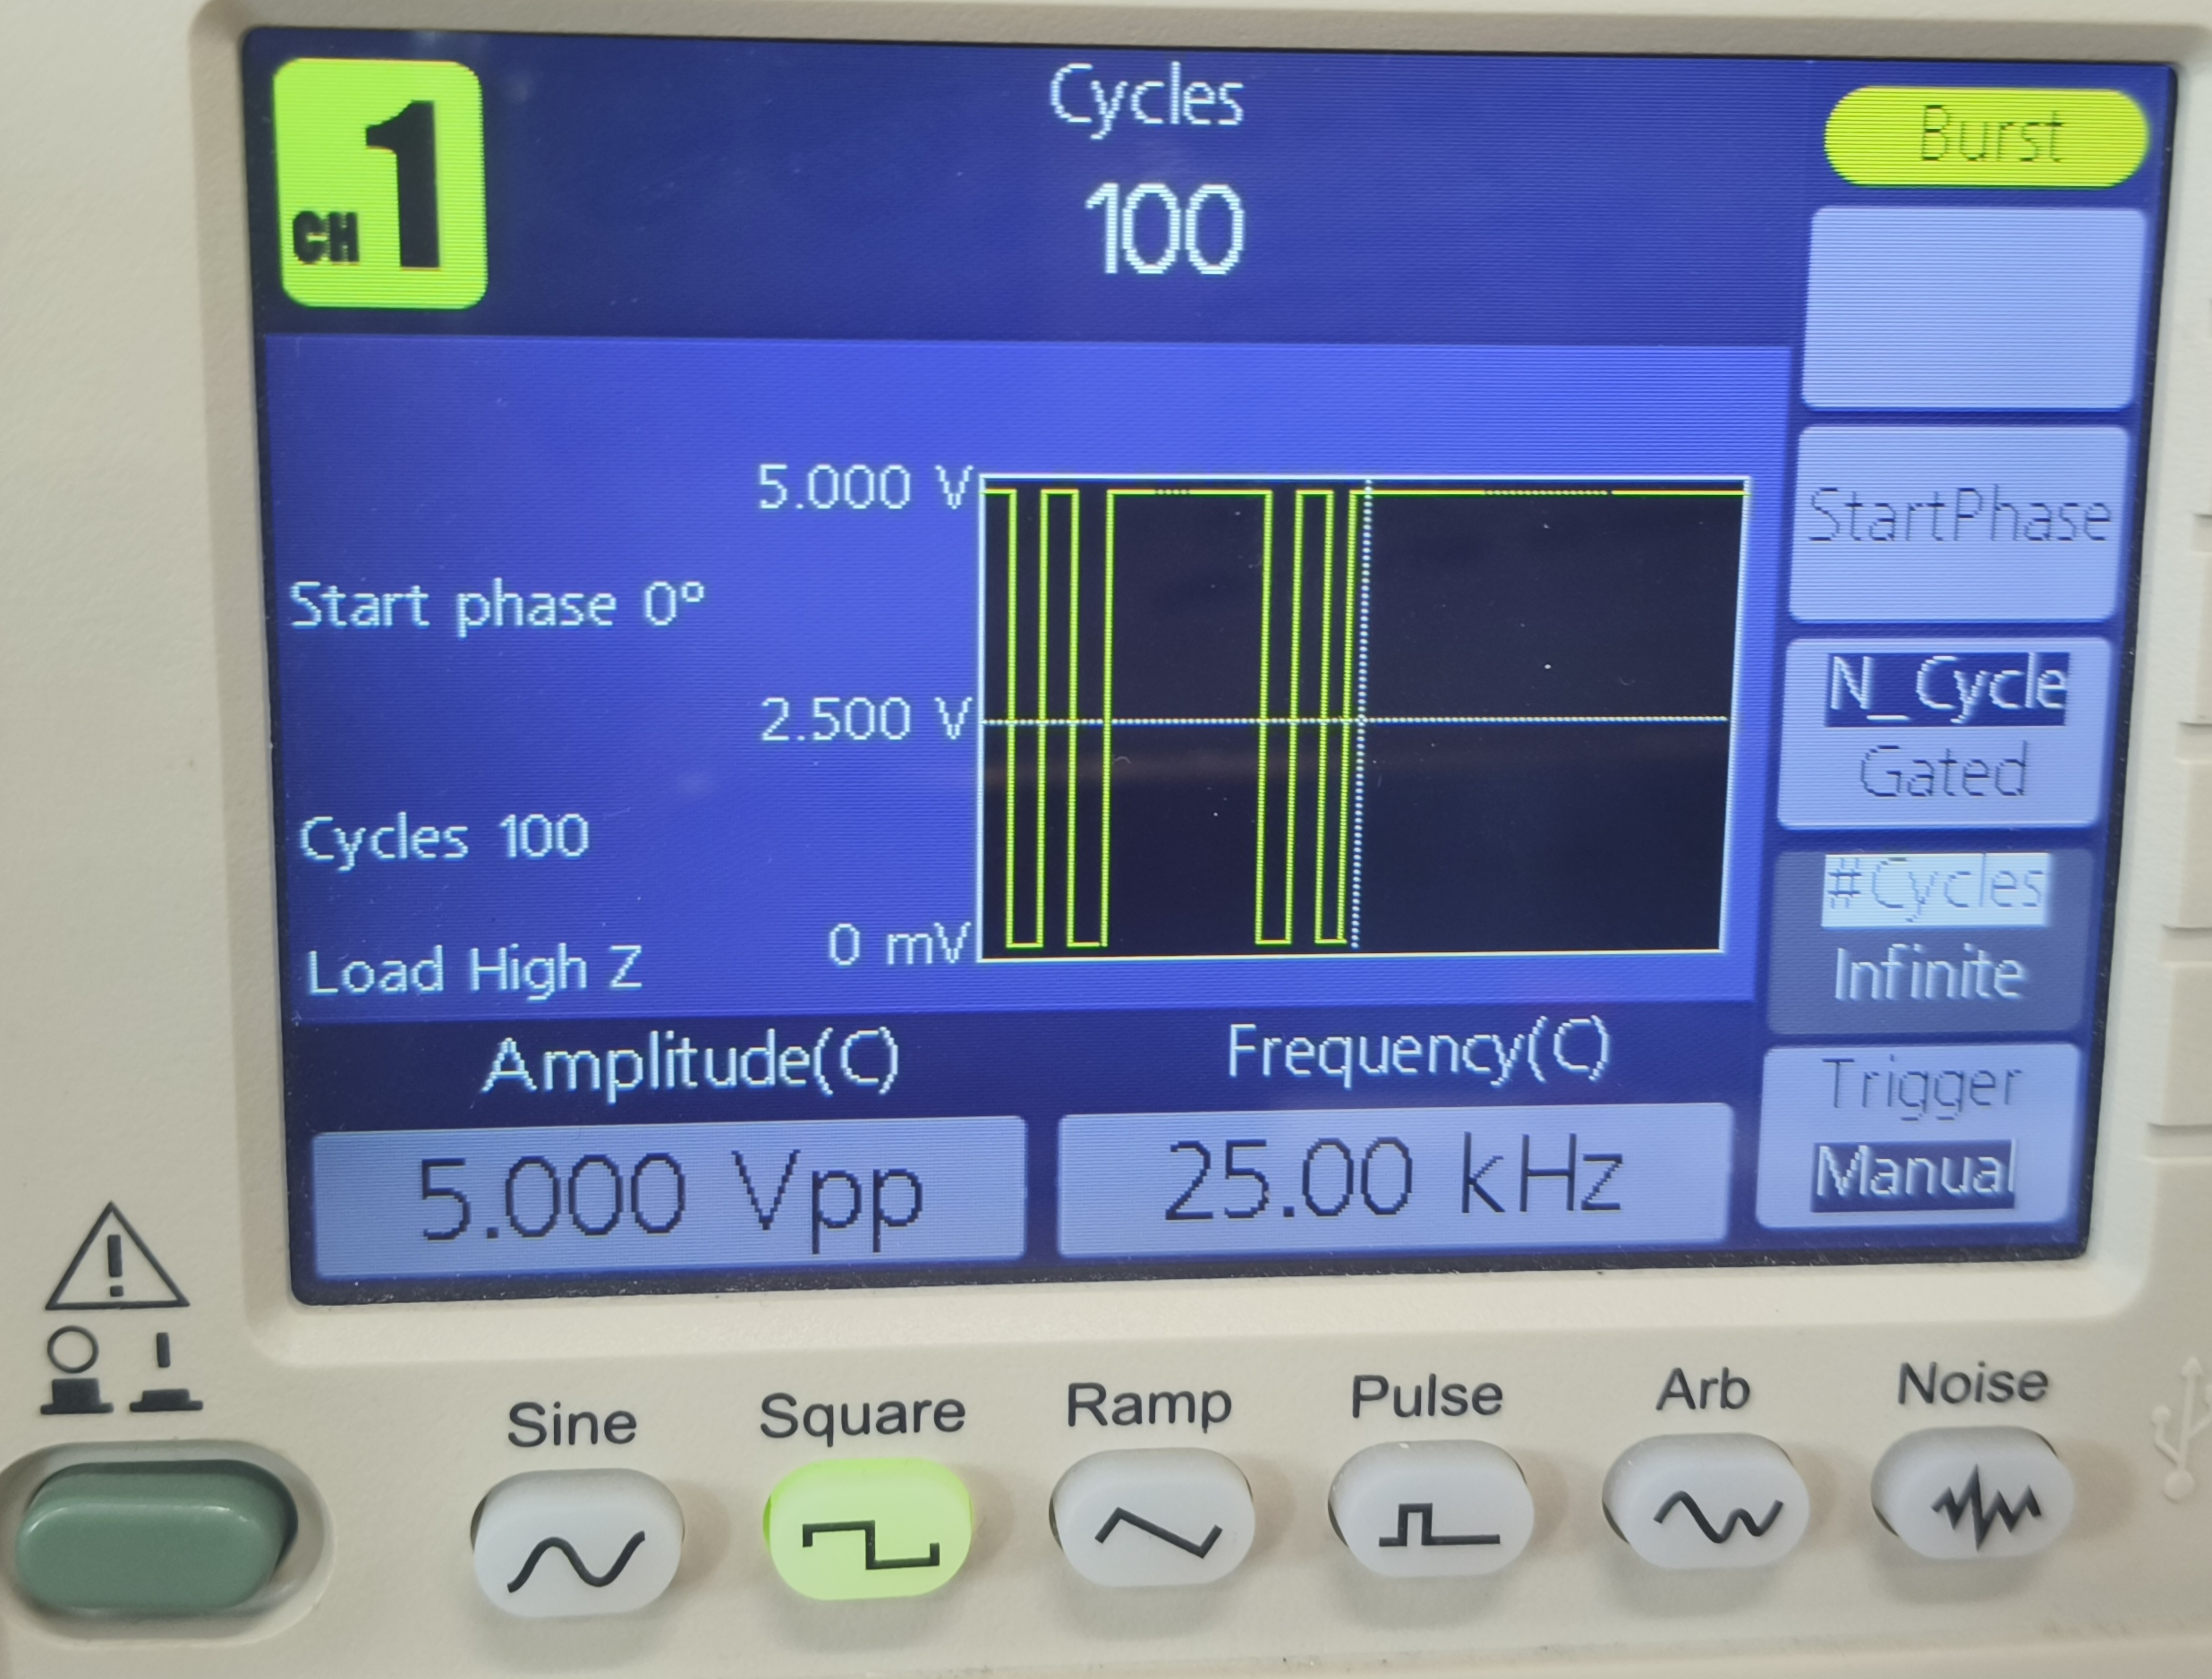
\includegraphics[width=\textwidth]{figs/t3_1.jpg} % Replace with the actual file name
        
    \end{minipage}
    \hfill
    \begin{minipage}[c]{0.48\textwidth}
        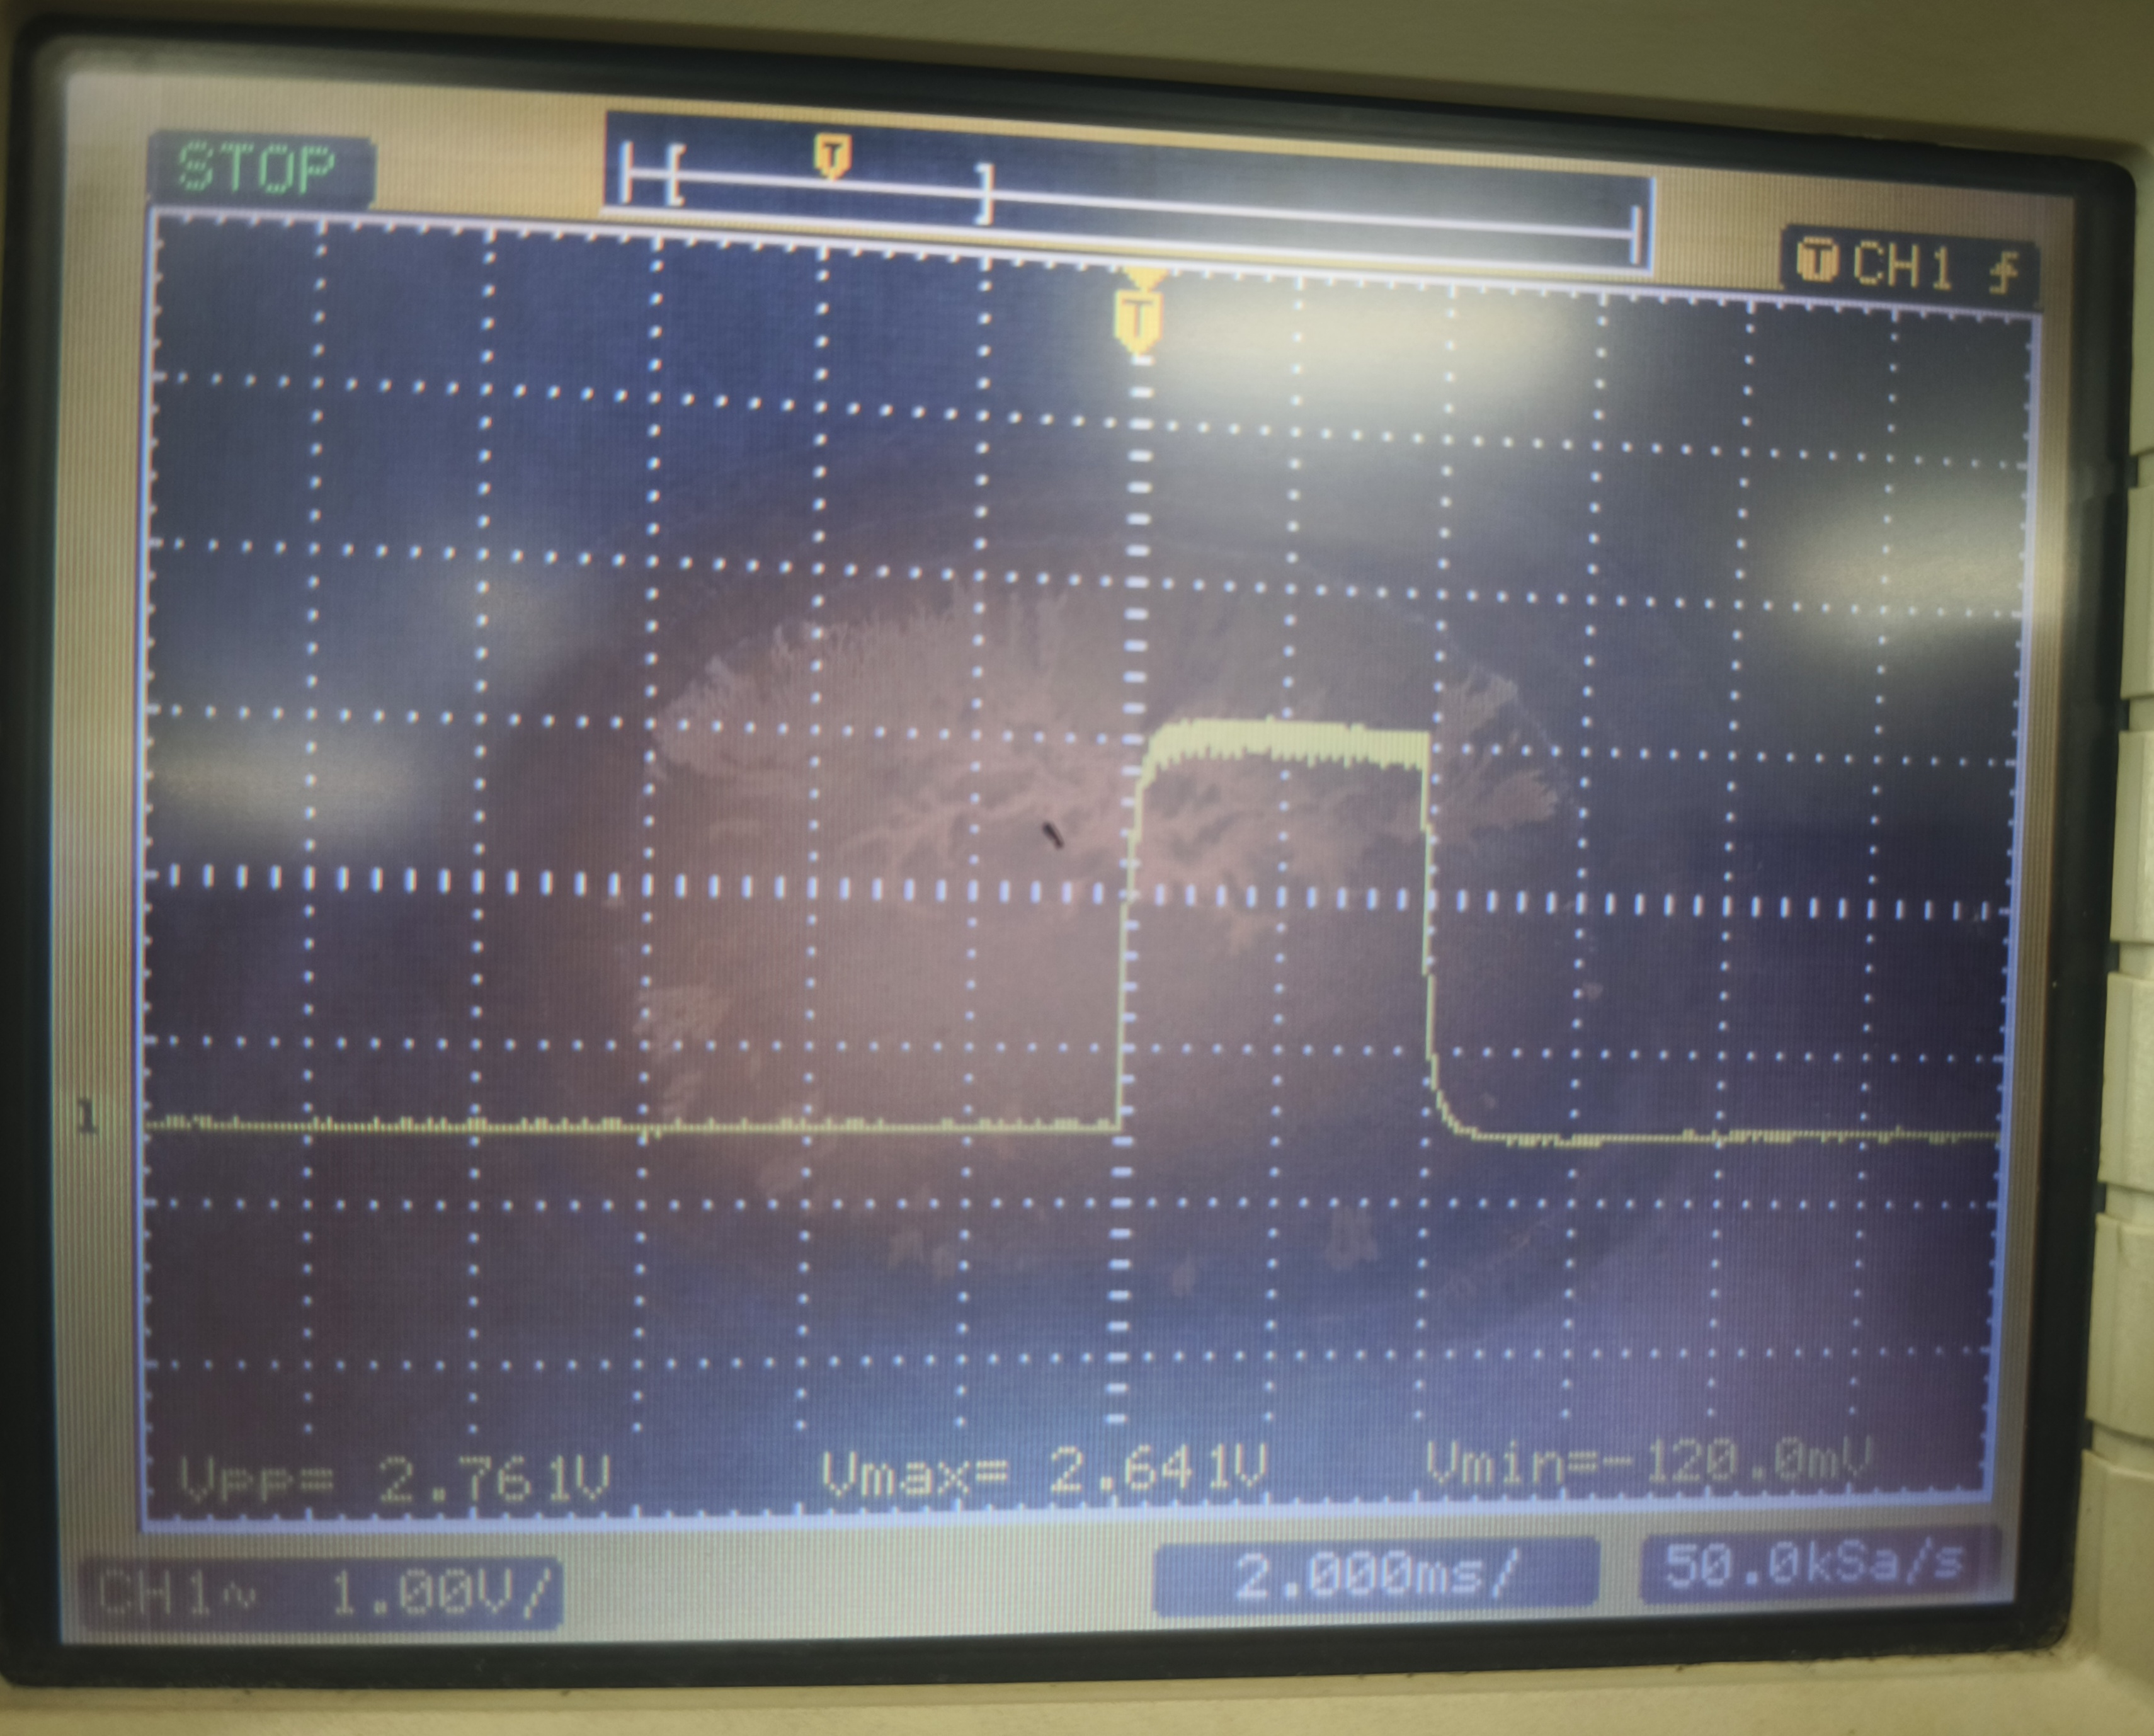
\includegraphics[width=\textwidth]{figs/tr3_1.jpg} % Replace with the actual file name
        
    \end{minipage}
    
\end{figure}
For Infinite Cycles
\begin{figure}[H] % H forces the figure to be placed exactly here
    \centering
    % Replace "1.jpg" with your actual image filename
    \begin{minipage}[c]{0.48\textwidth}
        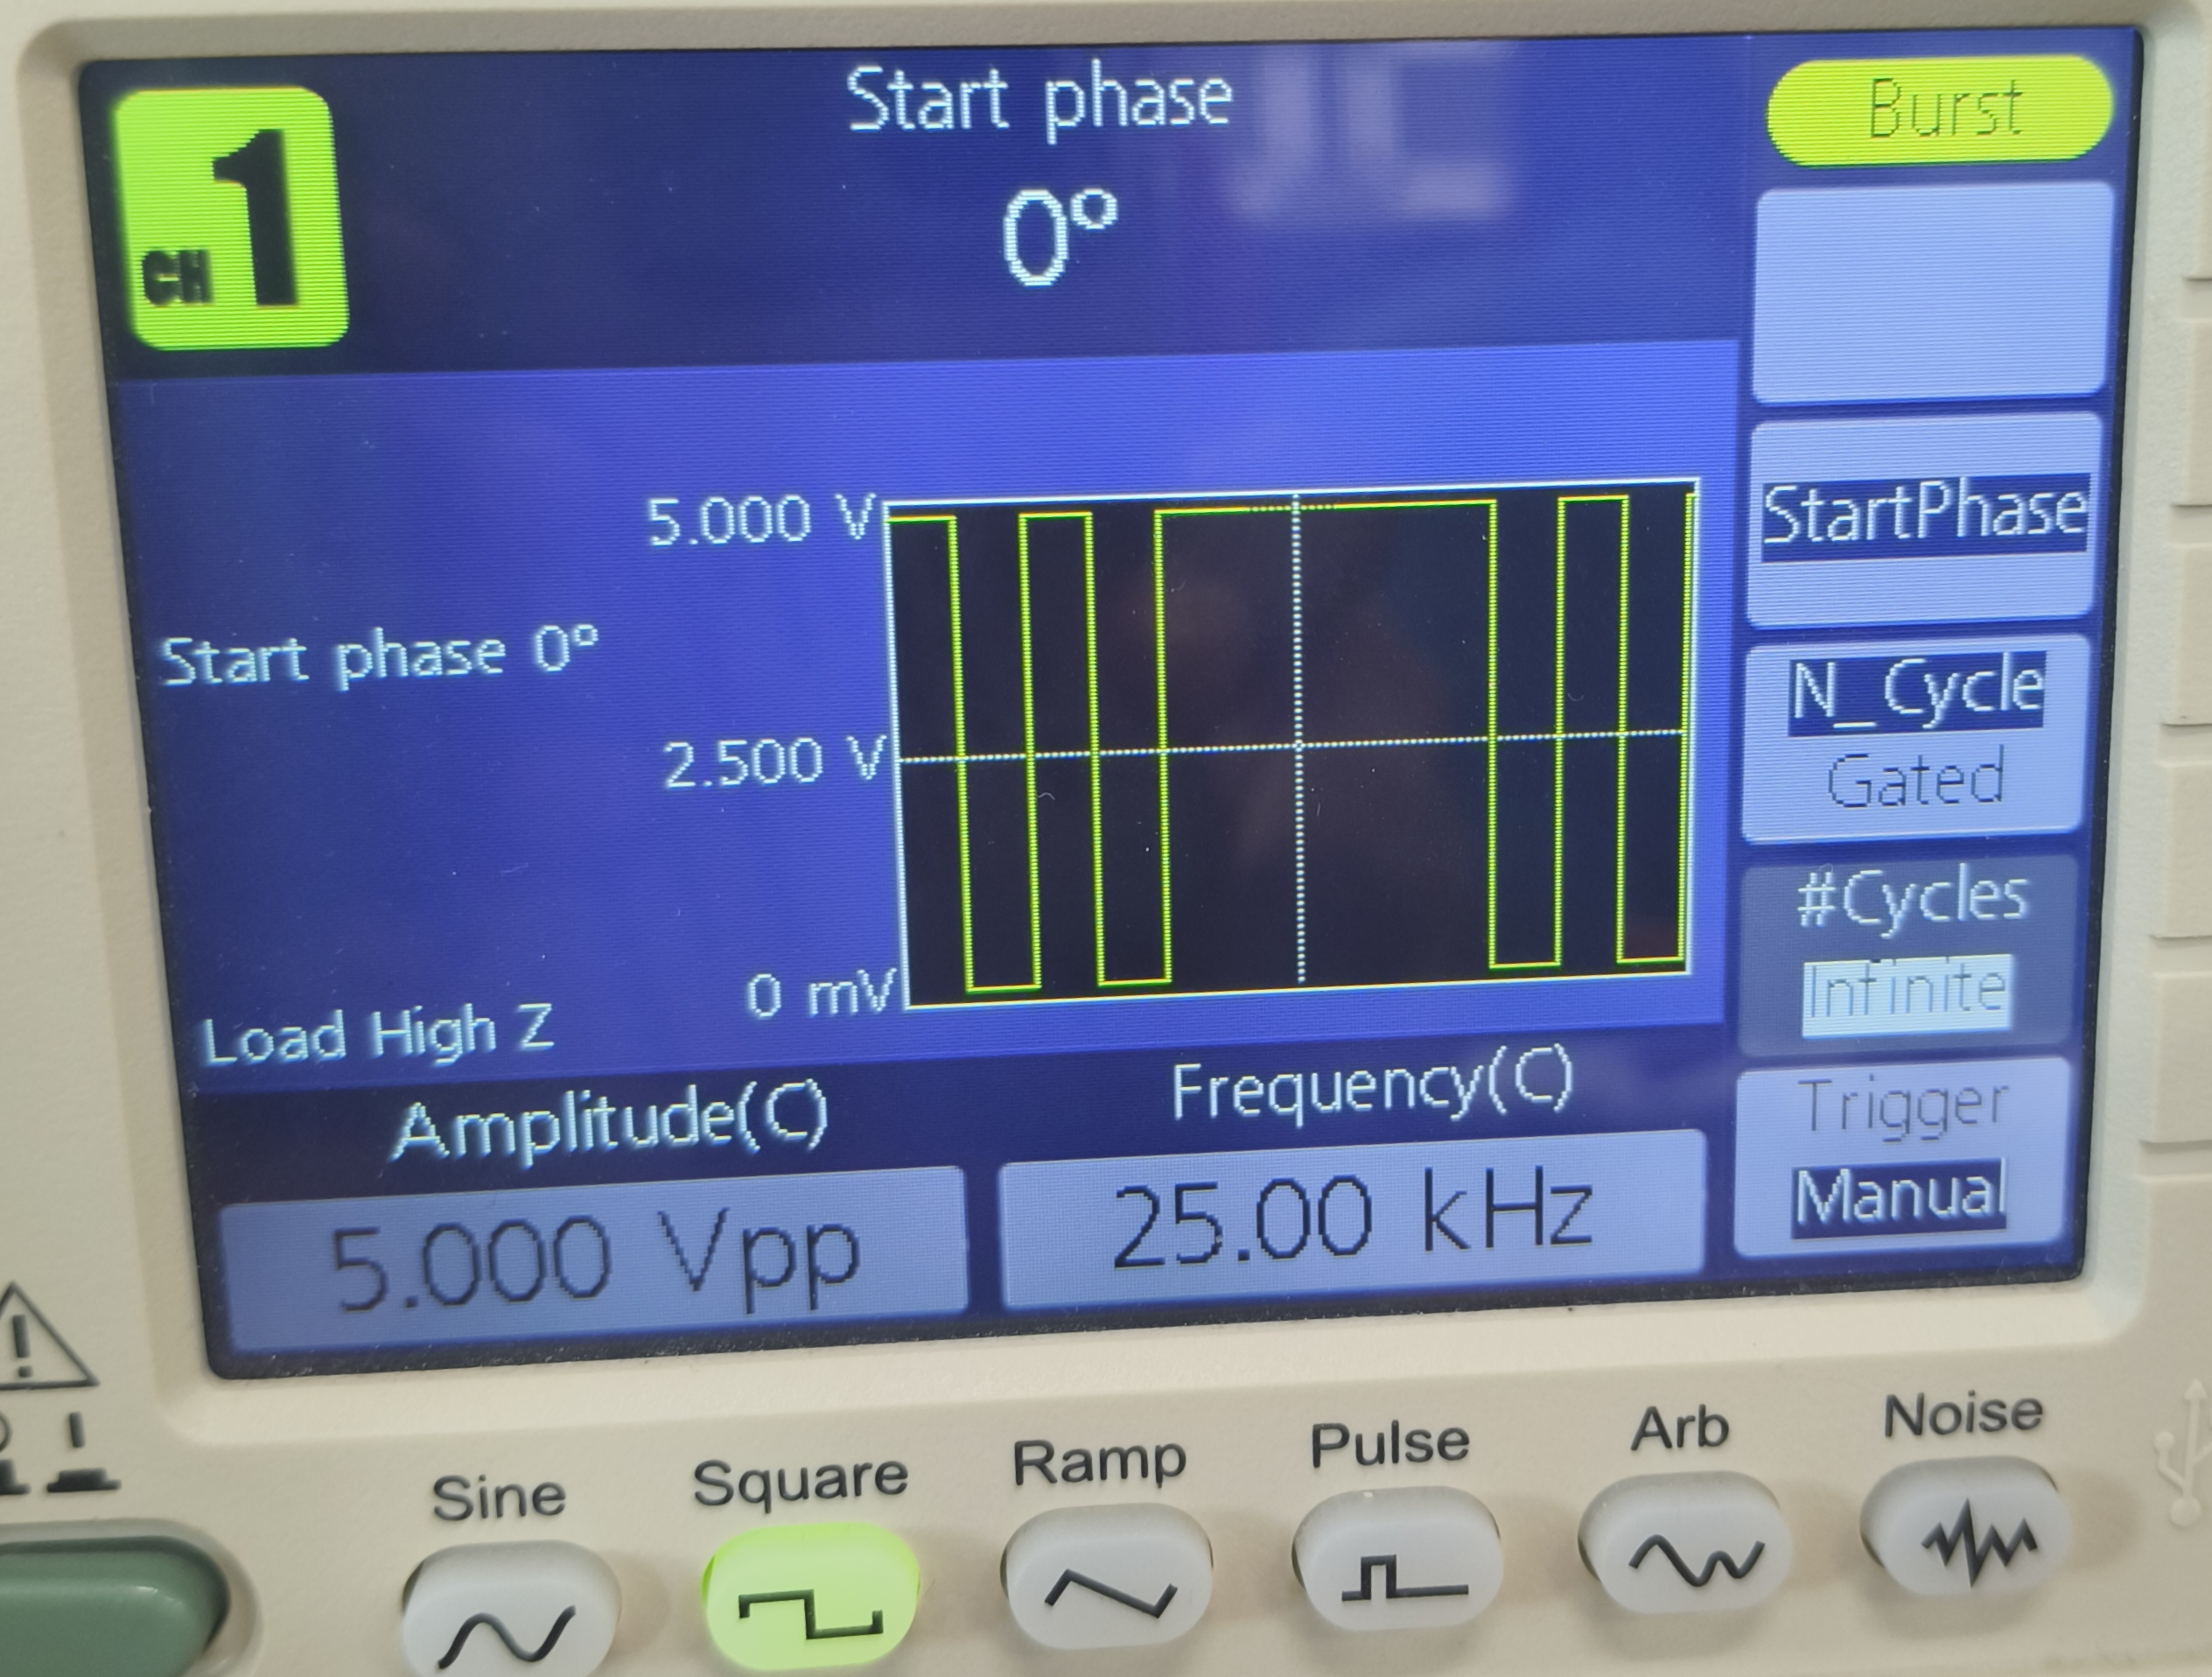
\includegraphics[width=\textwidth]{figs/t3_2.jpg} % Replace with the actual file name
        
    \end{minipage}
    \hfill
    \begin{minipage}[c]{0.48\textwidth}
        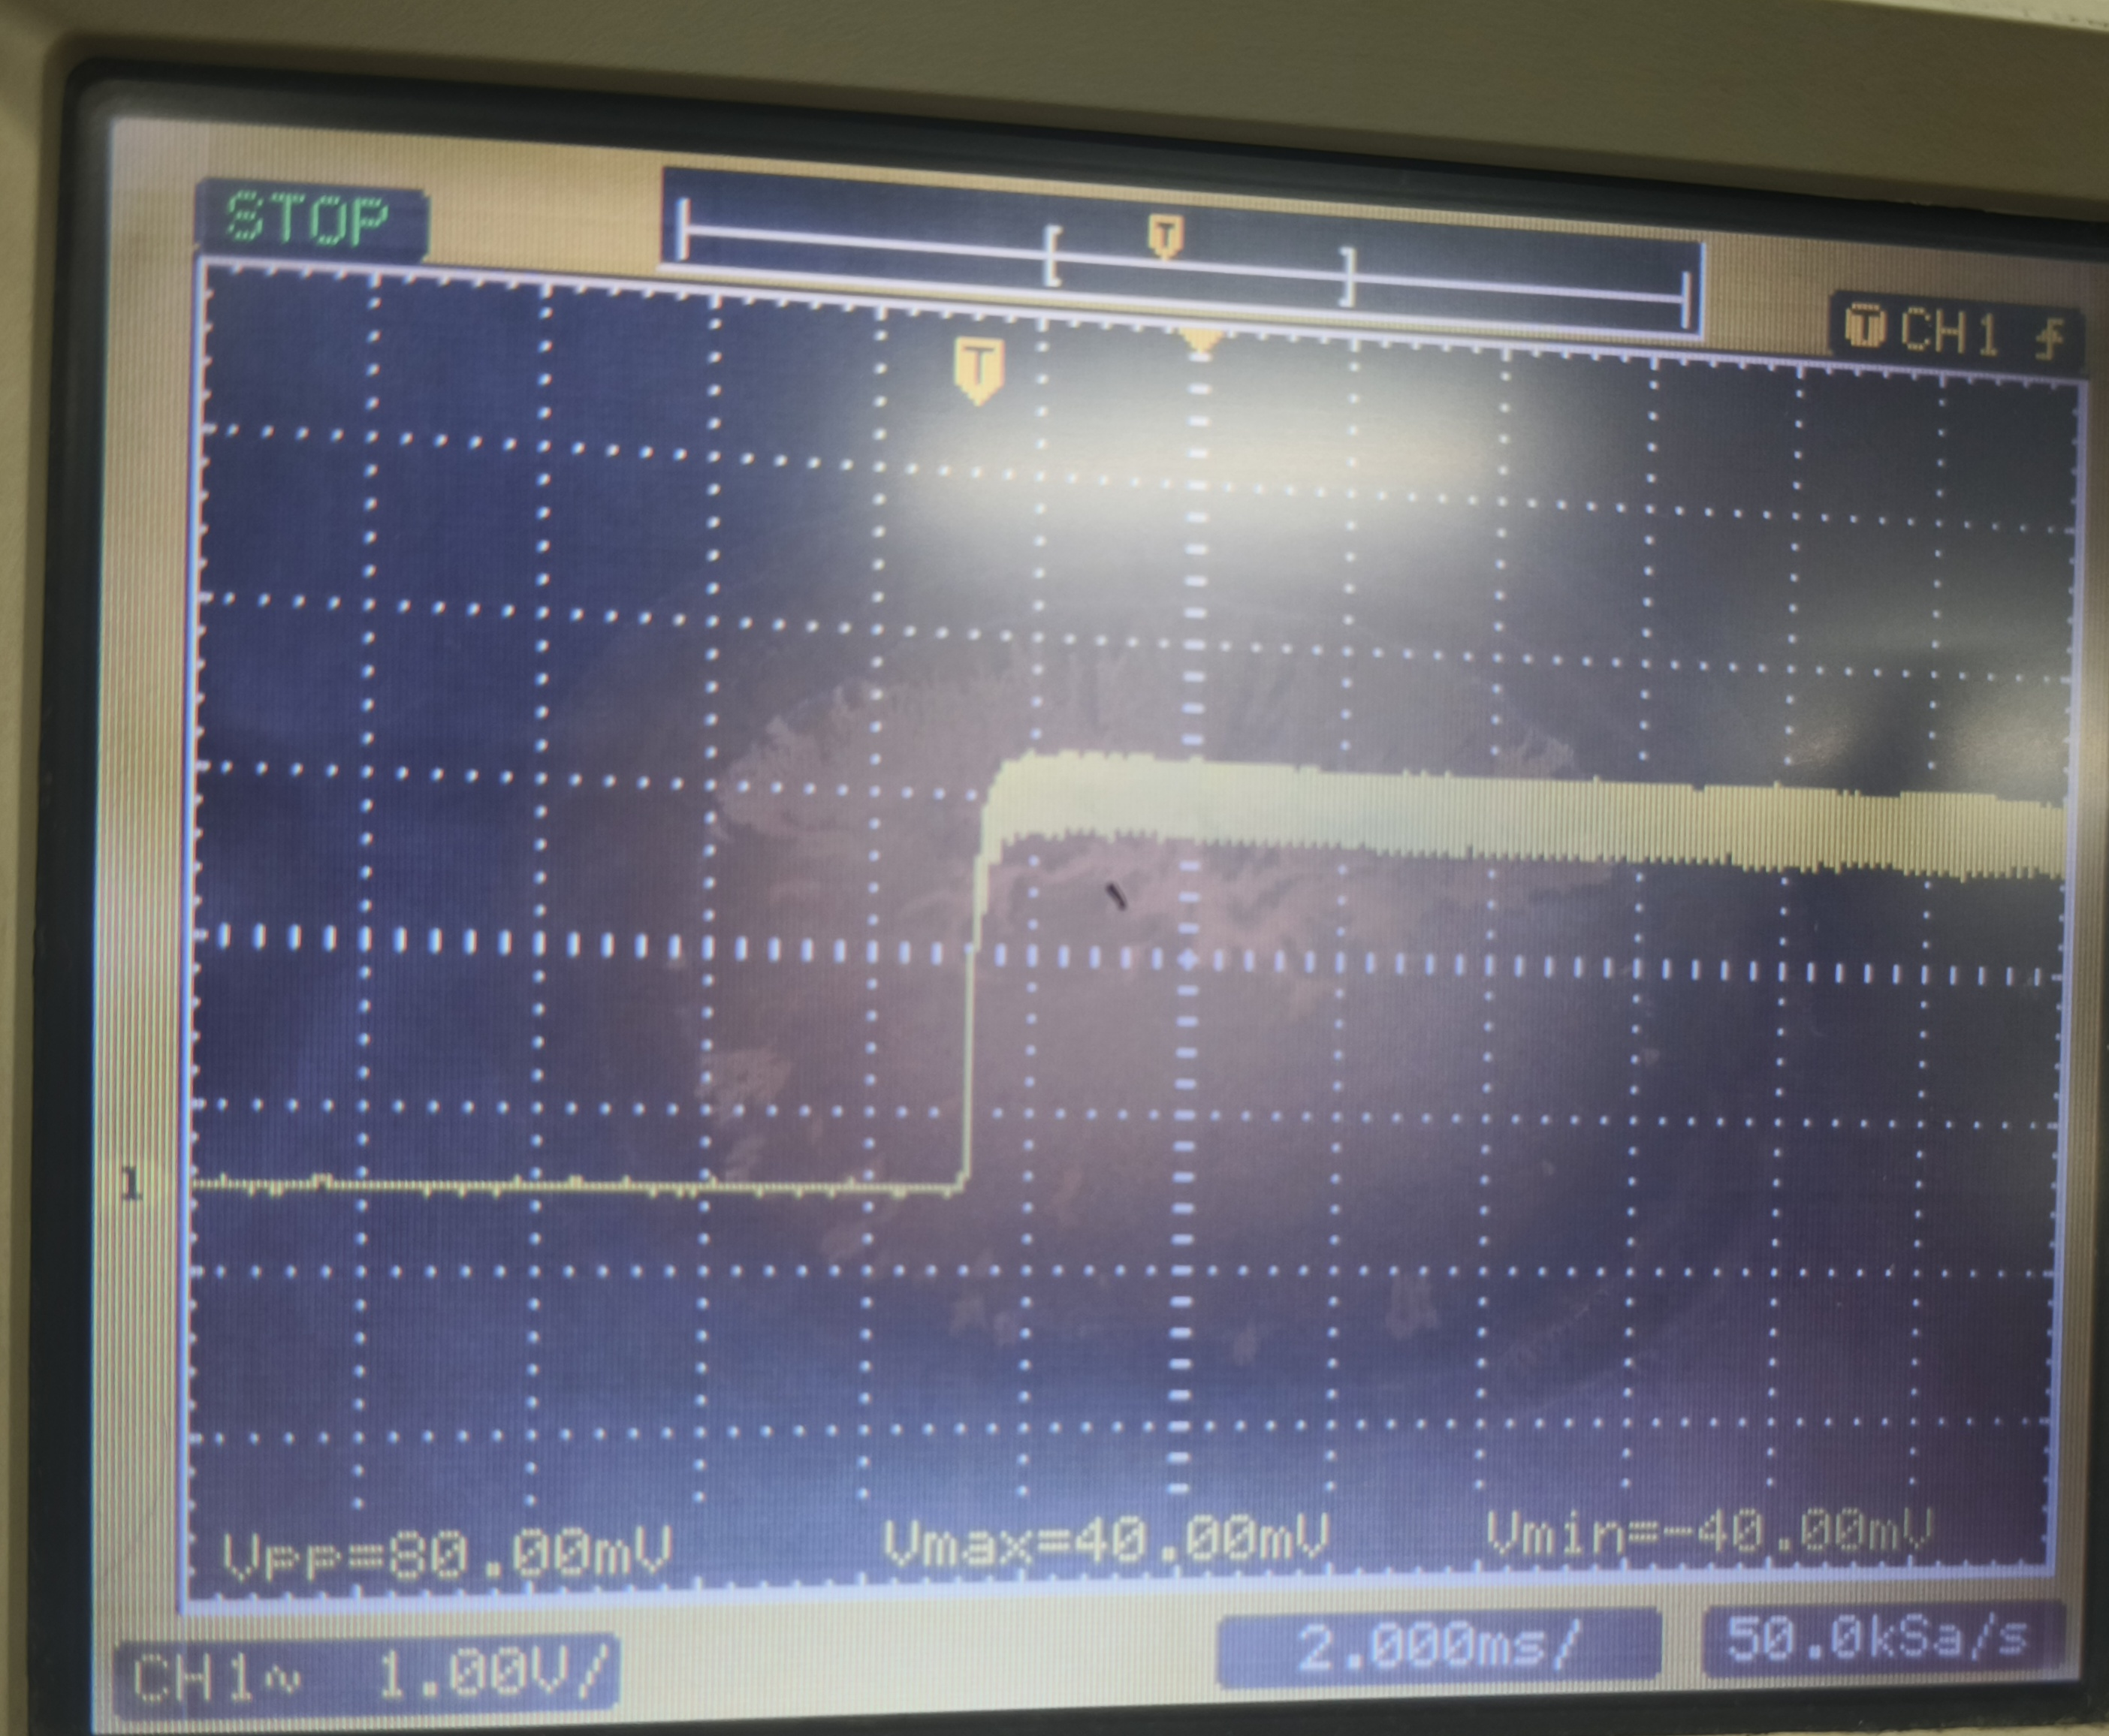
\includegraphics[width=\textwidth]{figs/tr3_2.jpg} % Replace with the actual file name
        
    \end{minipage}
    \caption{Transient $RC \gg T$}
    \label{fig:CRO-patterns}
\end{figure}
\begin{figure}
    \centering
    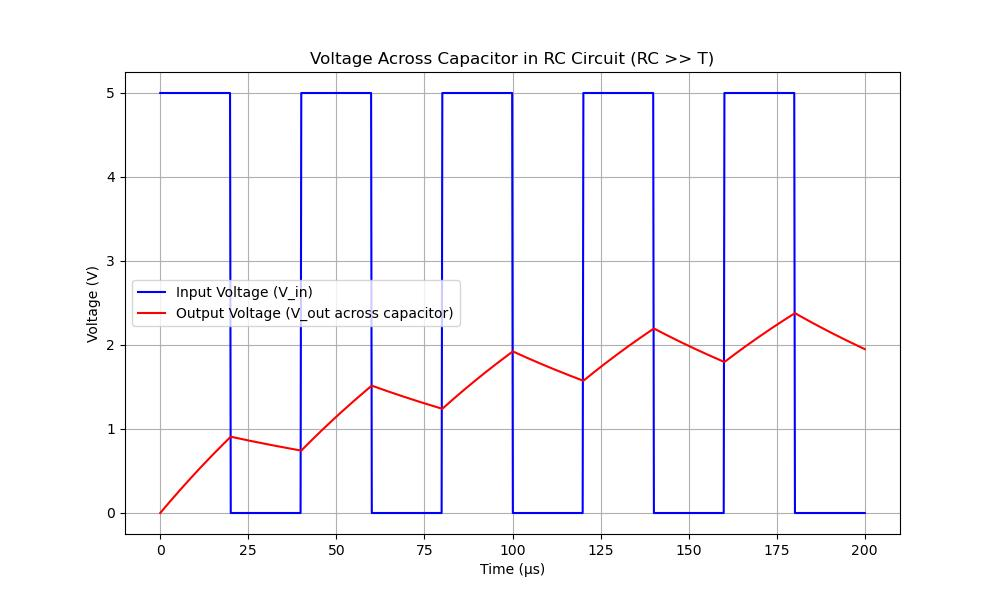
\includegraphics[width=\textwidth]{figs/3.jpg}
    \caption{Python $RC \gg T$}
    \label{fig:enter-label}
\end{figure}
    \item Steady-state response:
    \begin{figure}[H] % H forces the figure to be placed exactly here
    \centering
    % Replace "1.jpg" with your actual image filename
    \begin{minipage}[c]{0.48\textwidth}
        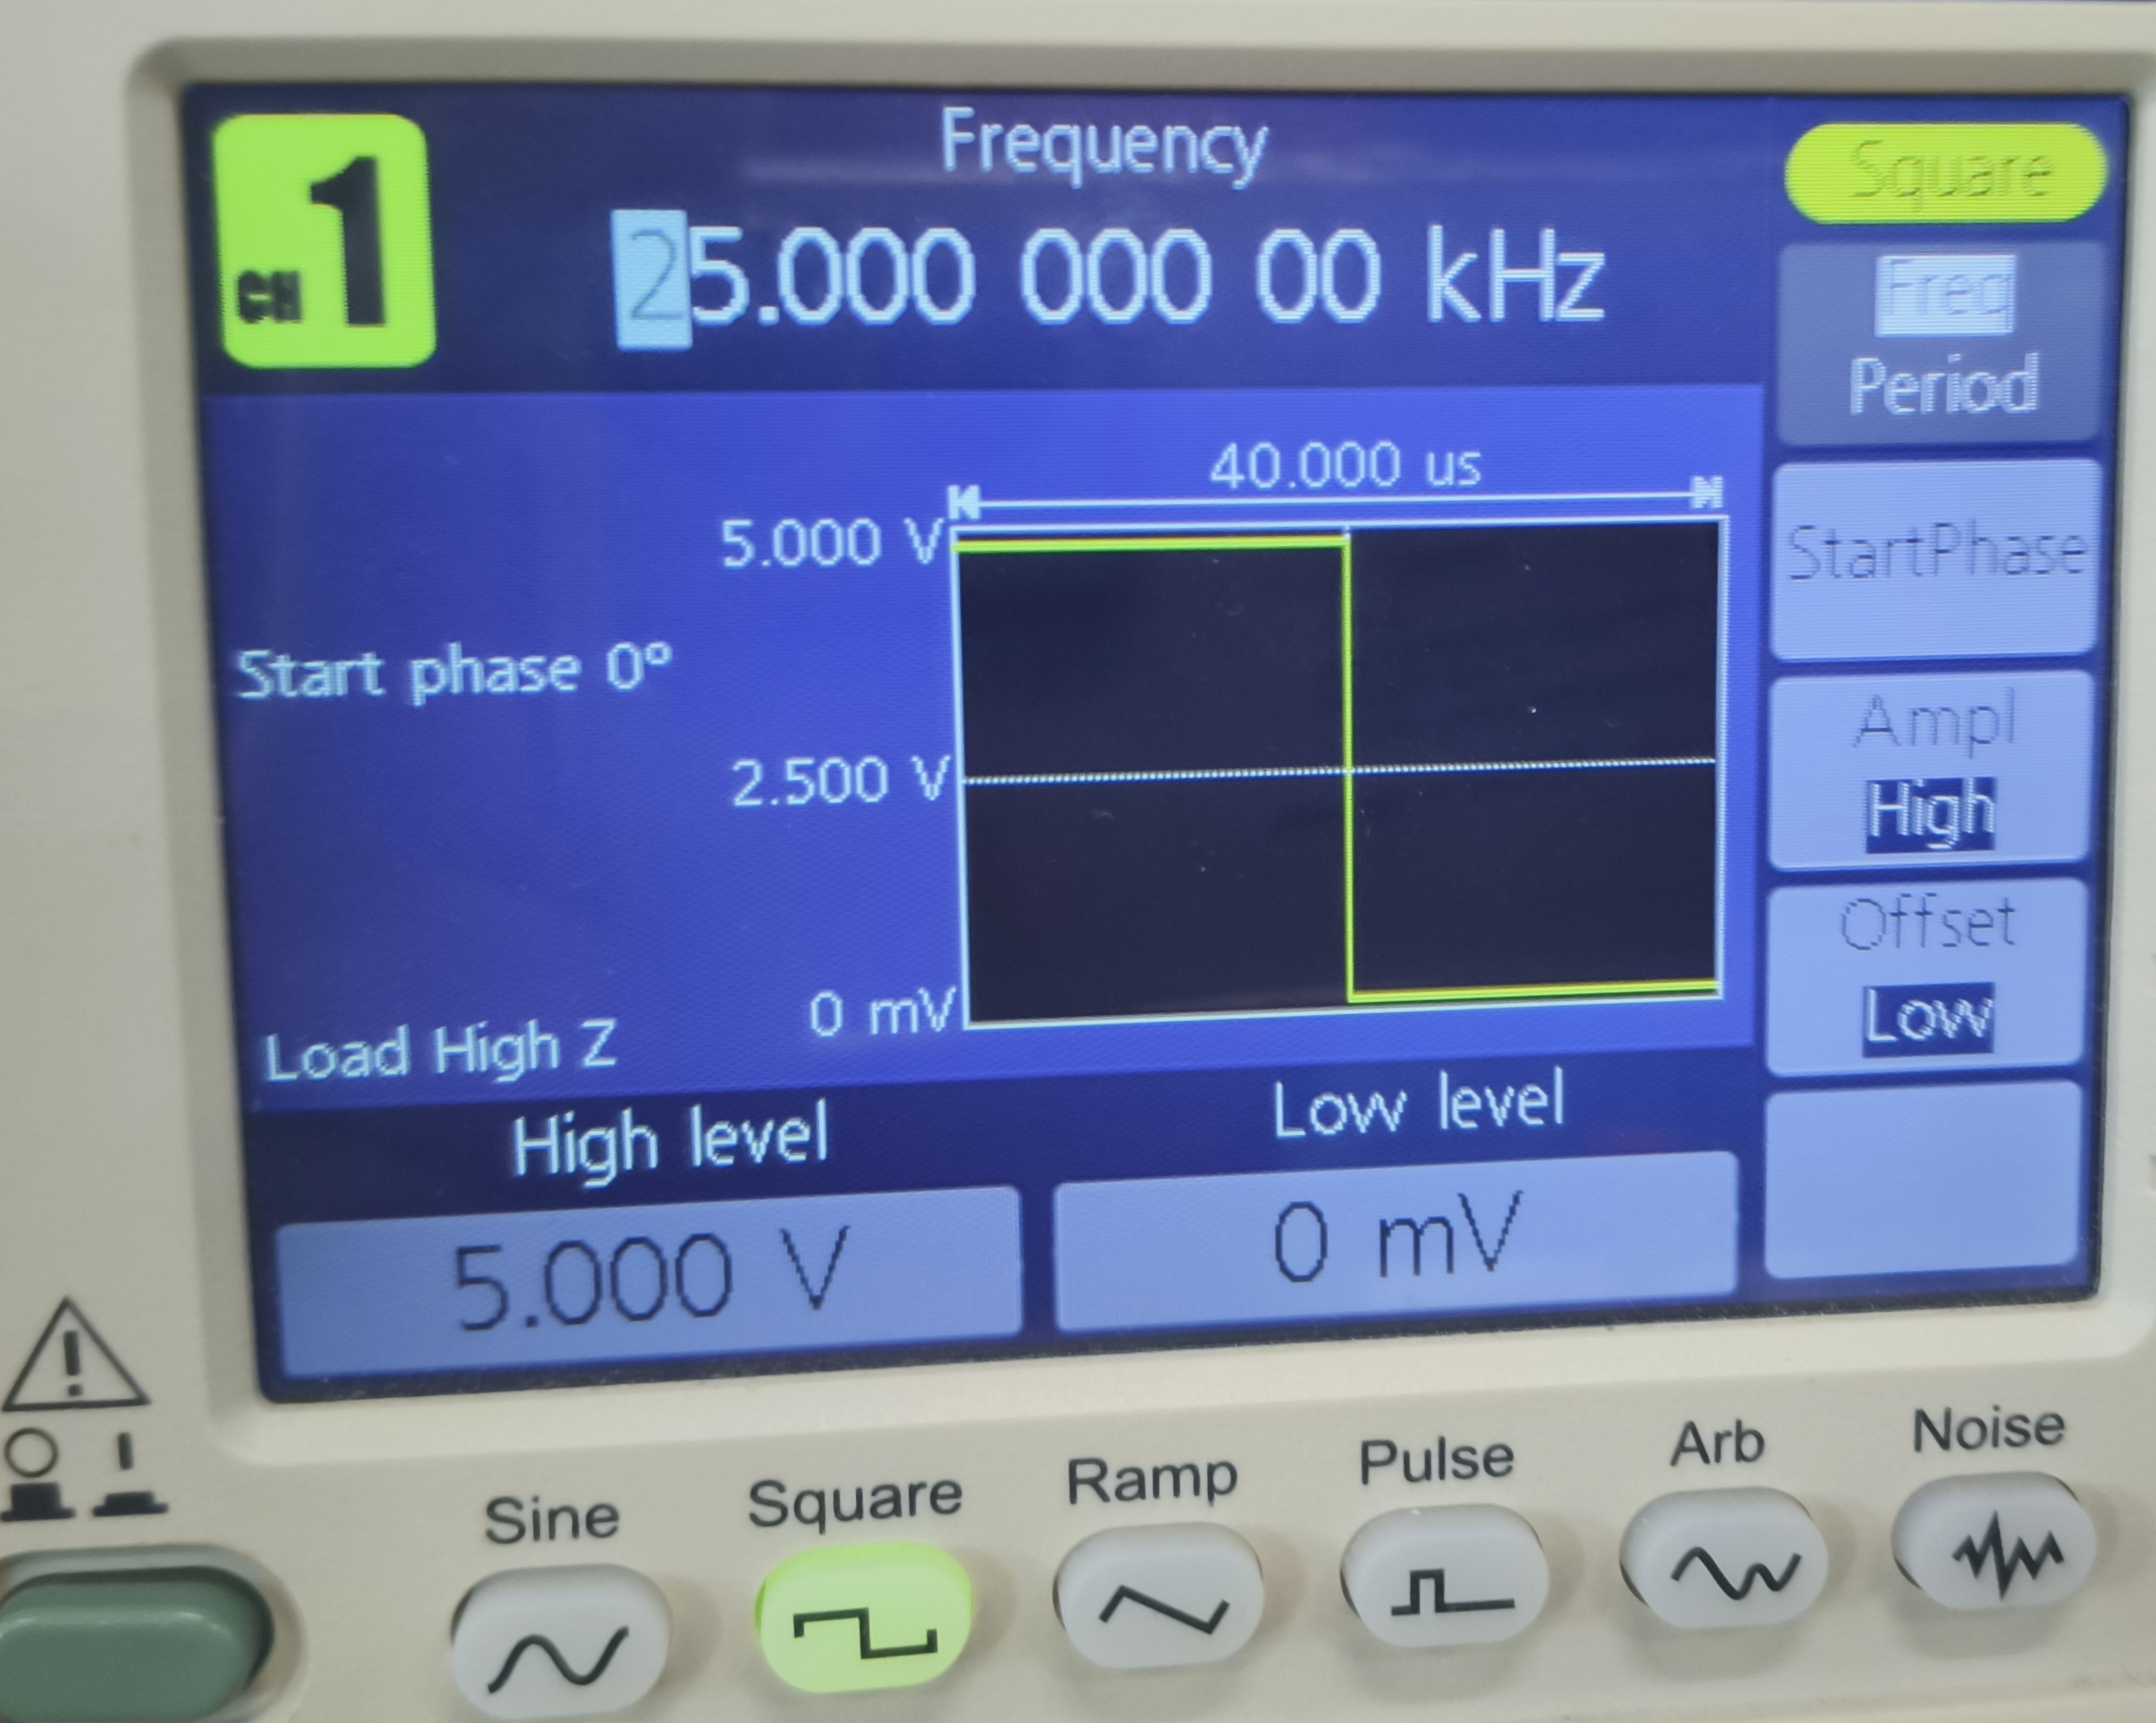
\includegraphics[width=\textwidth]{figs/s3.jpg} % Replace with the actual file name
        
    \end{minipage}
    \hfill
    \begin{minipage}[c]{0.48\textwidth}
        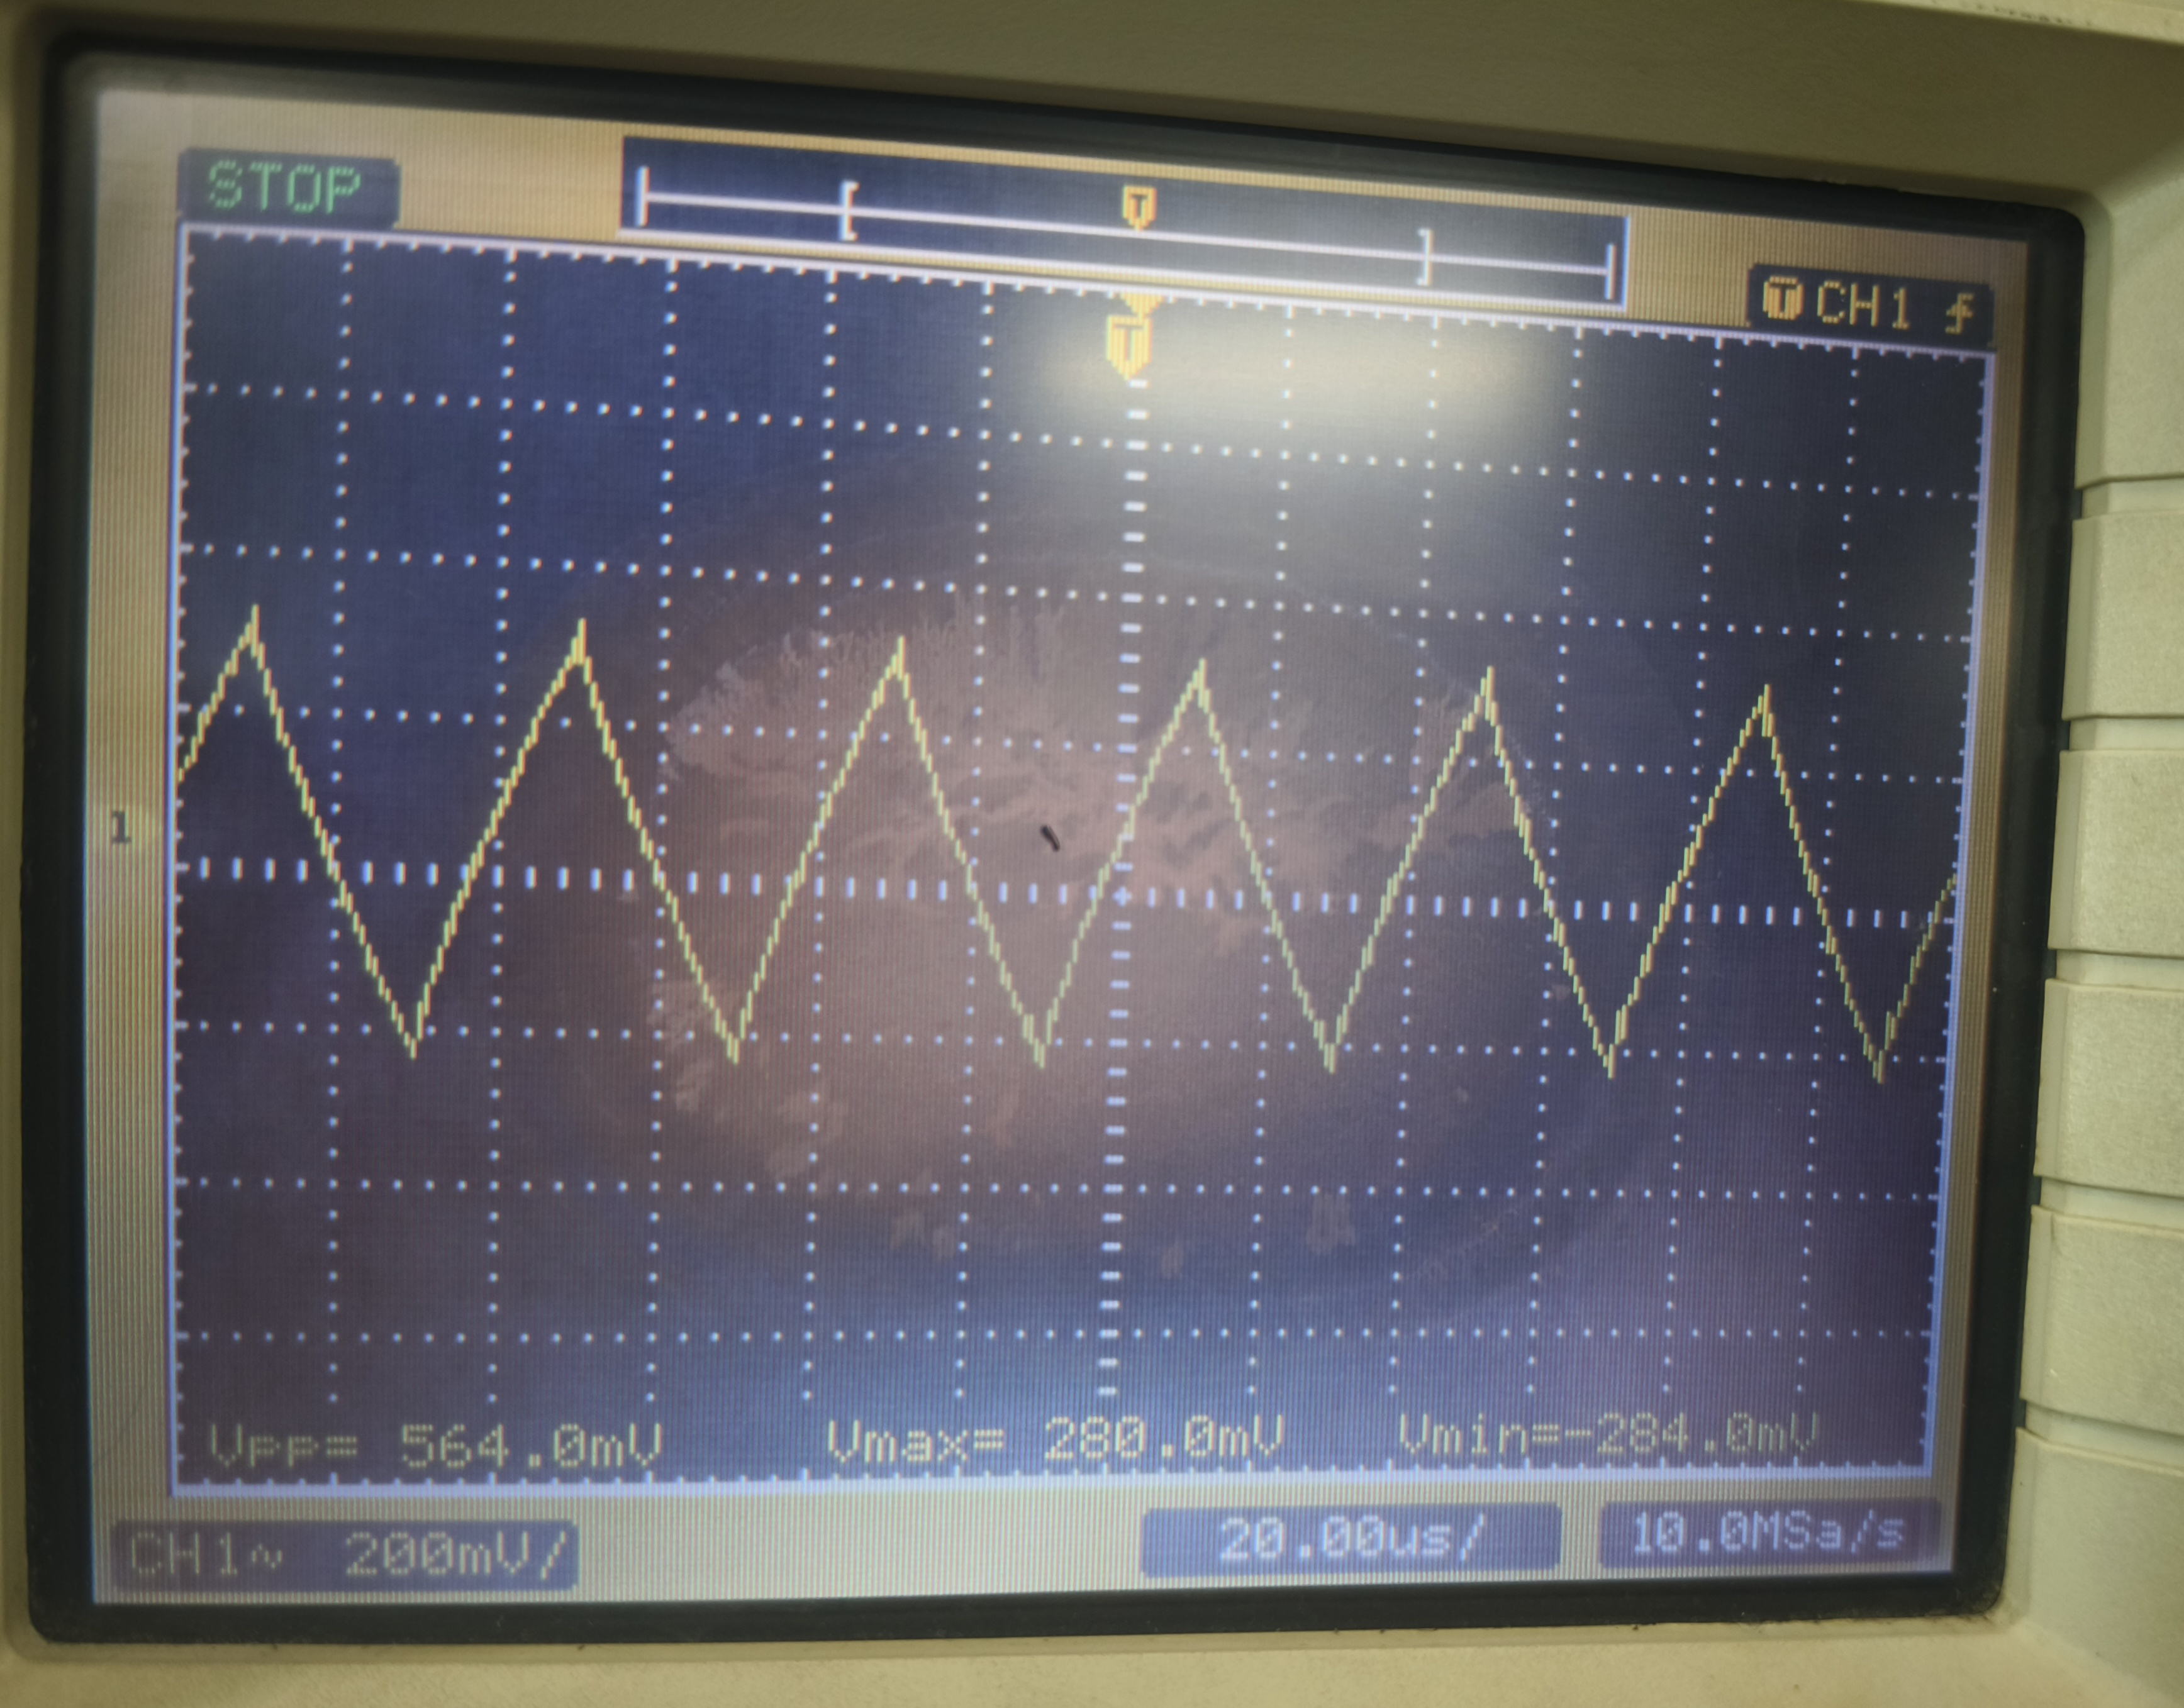
\includegraphics[width=\textwidth]{figs/sr3.jpg} % Replace with the actual file name
        
    \end{minipage}
    \caption{Steady State $RC \gg T$}
    \label{fig:CRO-patterns}
\end{figure}
\end{itemize}



\section{Conclusion}
In this document, we explored the step-by-step process of setting up an RC circuit on a breadboard and analyzed the voltage response across the capacitor when subjected to a square wave input. We derived the mathematical expressions governing the transient and steady-state behaviors of the circuit. The capacitor voltage follows an exponential pattern of charging and discharging, dictated by the circuit's time constant \( \tau = RC \). Understanding these concepts is essential for analyzing RC circuits in practical applications such as signal processing, filtering, and timing circuits.

\end{document}

